\chapter{Mathematical process model}
\label{chp:MathModel}

    \Eq{}{
        \Huge \frac{\partial}{\partial t}
    }

    The industrial scale production of highly pure oxygen and nitrogen as well as noble
    gases is still carried out by means of the cryogenic process.

    The initial process for production of pure oxygen first developed by Carl von Linde
    and first operated by Linde in 1902 \cite{Barron.1985} consisted of only
    a stripping section, in a way only half a rectification column. The reason for that is
    while it is easy to supply the heat necessary for the reboiler, a heat sink to operate
    a condenser at temperatures of about $95$ $K$ is not readily available on our planet.
    due to that highly pure oxygen could be withdrawn from the bottom of the column, but
    nitrogen was only produces at mediocre purities.

    The breakthrough that enabled operation of a ''full'' column, again developed by Linde in 1910,  was to operate the
    column sections at different pressures. That way the energy needed in the reboiler
    could be withdrawn from the condenser of the other column half. This leads to a
    somewhat inverted construction of the tower in comparison to regular distillation
    units, because the lower section forms the top section in this case and condenser
    and reboiler usually at the top and bottom of a column are combined in a single
    heat exchange unit in the middle of the column. This specialty of the process also
    leads to the need that the absolute values of the energies used in condenser and
    reboiler need to be equal. On terms of modelling the process this also forms a
    considerable challenge.

    \begin{figure}
        \begin{tikzpicture}
    \draw [arrow] (-4,0) -- (-2,0) node [pos=0.5,above] {} ;
    \draw [line width=1pt] (-2,0.75) rectangle (1,-0.75) node [align=center] at (-0.5,0) {\footnotesize pre- \\ \footnotesize purification} ;
    \draw [arrow] (1,0) -- (3,0) ;
    \draw [line width=1pt] (3,0.75) rectangle (6,-0.75) node [align=center] at (4.5,0) {\footnotesize compression \\ \footnotesize \& liquefaction};
    \draw [arrow] (6,0) -- (8,0) ;
    \draw [line width=1pt] (8,0.75) rectangle (11,-0.75) node at (9.5,0) {\footnotesize purification} ;
    \draw [arrow] (11,0) -- (13,0) ;
\end{tikzpicture}

        \caption{simplified cryogenic air separation process.}
        \label{fig:asu_simple}
    \end{figure}

    A simplified overview of the major process steps is given in \reffig{fig:asu_simple}.
    Within the following sections the different process steps will be discussed in more detail.
    When appropriate the mathematical model for single process units is discussed as well.
    In addition to the separate process steps displayed in \reffig{fig:asu_simple} the aspect
    of heat integration os essential to successfully operating an air separation unit (ASU).
    This aspect will be discussed separately as well (\refsec{sec:heat_exchange})

    The pre-purification step of the process aim to reduce the amount of unwanted impurities
    from the ambient air as far as possible. The main sources of contamination are in this case
    dust and other organic components that can be found depending on the time of year and
    location of the plant. Furthermore are water and carbon dioxide common components in
    ambient air. The removal of these components is undertaken by means of adsorption molecular
    sieves such as zeolite or for initial steps coarser sieves. However the design and simulation
    of these pre-purification measures is not within the scope of this work. For more information
    the interested reader is referred to \cite{Acharya.1996}.


\section{Purification}
\label{sec:SteadyStateModel}
    The purification of the liquefied gases is performed by distillation columns
    operated at different pressure.
    These distillation columns form the heart of the air separation process and their
    operation parameters are crucial in terms of enabling the desired separation.
    While the aspect of heat integration poses is also essential in terms of profitability of
    the process.

    Subsequently this section is concerned with the description of different aspects of
    modeling distillation columns. First the mathematical model will be presented in
    more detail. Afterwards the handling of different specifications for individual
    columns is elaborated upon. Lastly the issue of initializing the respective models
    and the implemented solution is presented.

\subsection{Distillation column model}
\label{sec:SSM:dist}

    In this section the working equations used to model the different distillation
    columns in the process, known as the MESH equations, are given. These equations,
    although rather plain at first glimpse, form a set of highly non-linear, highly
    coupled equations. The solutions of these equations is not a trivial
    task for current solution algorithms, whose success is highly dependent on the
    quality of initial guesses provided. Therefore a strategy used for the automated
    generation of such guesses will be described as well.

    \begin{figure}
        \centering
        \begin{subfigure}{0.3\textwidth}
            \centering
            \begin{tikzpicture}[arrow2/.style={line width=0.5pt,->,>=latex,gray},scale=0.52]
    \draw [line width=0.5pt,gray] (1,4.8) -- (-1,4.8) node [above,pos=0.5,black,yshift=-1mm] {\scriptsize 2};
    \draw [line width=0.5pt,gray] (1,-4.8) -- (-1,-4.8) node [above,pos=0.5,black,yshift=-1mm] {\scriptsize N-1};
    \draw [line width=0.5pt,gray] (1,-4.0) -- (-1,-4.0) node [above,pos=0.5,black] {};
    \draw [line width=0.5pt,gray] (1,-3.2) -- (-1,-3.2) node [above,pos=0.5,black] {};
    \draw [line width=0.5pt,gray] (1,-0.8) -- (-1,-0.8) node [above,pos=0.5,black] {};
    \draw [line width=0.5pt,gray] (1,0.0) -- (-1,0.0) node [above,pos=0.5,black] {};
    \draw [line width=0.5pt,gray] (1,0.8) -- (-1,0.8) node [above,pos=0.5,black] {};
    \draw [line width=0.5pt,gray] (1,1.6) -- (-1,1.6) node [above,pos=0.5,black] {};
    \draw [line width=0.5pt,gray] (1,-1.6) -- (-1,-1.6) node [above,pos=0.5,black] {};
    \draw [line width=1pt, rounded corners] (-1.0,2.8) -- (-1.0,5) .. controls (-0.8,5.8) and (0.8,5.8) .. (1.0,5) node (a) [inner sep=0cm , pos=0.5] {} -- (1.0,2.8);
    \draw [arrow] (a) -- (0,6.2) -- (2.5,6.2) node [draw, line width=1pt, pos=1, circle, minimum size=0.9cm, fill=white] {} -- (2.5,4.8) -- (1,4.8) ; % condenser
    \draw [line width=0.5pt] (4,6.5) -- (2.2,6.5) -- (2.6,6.2) -- (2.2,5.9) -- (4,5.9) ;   % heater condenser
    \draw [line width=1pt] (1.0,2.6) .. controls (0.75,2.85) and (0.25,2.85) .. (0.0,2.6) .. controls (-0.25,2.35) and (-0.75,2.35) .. (-1.0,2.6);
    \draw [line width=1pt] (1.0,-2.2) .. controls (0.75,-2.45) and (0.25,-2.45) .. (0.0,-2.2) .. controls (-0.25,-1.95) and (-0.75,-1.95) .. (-1.0,-2.2);
    \draw [line width=1pt] (1.0,2.8) .. controls (0.75,3.05) and (0.25,3.05) .. (0.0,2.8) .. controls (-0.25,2.55) and (-0.75,2.55) .. (-1.0,2.8);
    \draw [line width=1pt] (1.0,-2.4) .. controls (0.75,-2.65) and (0.25,-2.65) .. (0.0,-2.4) .. controls (-0.25,-2.15) and (-0.75,-2.15) .. (-1.0,-2.4);
    \draw [line width=1pt] (1.0,2.6) -- (1.0,-2.2) ;
    \draw [line width=1pt] (-1.0,2.6) -- (-1.0,-2.2) ;
    \draw [line width=1pt, rounded corners] (1.0,-2.4) -- (1.0,-5) .. controls (0.8,-5.8) and (-0.8,-5.8) .. (-1.0,-5) node (b) [inner sep=0cm , pos=0.5] {} -- (-1.0,-2.4) ;
    \draw [arrow] (b) -- (0,-6.2) -- (2.5,-6.2) node [draw, line width=1pt, pos=1, circle, minimum size=0.9cm, fill=white] {} -- (2.5,-4.8) -- (1,-4.8) ;
    \draw [line width=0.5pt] (4,-6.5) -- (2.2,-6.5) -- (2.6,-6.2) -- (2.2,-5.9) -- (4,-5.9) ; % heater reboiler
    \draw [arrow2] (2.0,-4.8) -- (2.0,-4.0) -- (1.0,-4.0) ;
    \draw [arrow2] (2.0,-4.0) -- (2.0,-3.2) -- (1.0,-3.2) ;
    \draw [arrow2] (-2.0,0.8) -- (-2.0,1.6) -- (-1.0,1.6) ;
    \draw [arrow2] (-2.0,0.8) -- (-2.0,0.0) -- (-1.0,0.0) ;
    \draw [arrow2] (-2.0,0.0) -- (-2.0,-0.8) -- (-1.0,-0.8) ;
%    \draw [arrow2] (-2.0,-0.8) -- (-2.0,-1.6) -- (-1.0,-1.6) ;
%    \draw [arrow2] (1.0,-0.8) -- (2.0,-0.8) ;
    \draw [arrow2] (1.0,0.0) -- (2.0,0.0) ;
    \draw [arrow2] (1.0,0.8) -- (2.0,0.8) ;
%    \draw [arrow2] (1.0,1.6) -- (2.0,1.6) ;
    \draw [arrow2] (1.0,-1.6) -- (2.0,-1.6) ;
    \draw [line width=0.5pt,gray] (2.0,0.8) -- (2.0,-1.6) ;
    \draw [line width=0.5pt,gray,dotted] (-2.0,1.6) -- (-2.0,2.2) ;
    \draw [line width=0.5pt,gray,dotted] (-2.0,-0.8) -- (-2.0,-1.4) ;
    \draw [line width=0.5pt,gray,dotted] (2.0,0.8) -- (2.0,1.4) ;
    \draw [line width=0.5pt,gray,dotted] (2.0,-1.6) -- (2.0,-2.2) ;
    \draw [line width=0.5pt,gray,dotted] (2.0,-3.2) -- (2.0,-2.6) ;
    \draw [arrow] (2.5,4.8) -- (4,4.8) ;
    \draw [arrow] (2.5,-4.8) -- (4,-4.8) ;
    \draw [arrow] (-3.0,0.8) -- (-1.0,0.8) ;
    \draw [arrow] (1.0,-0.8) -- (3.0,-0.8) ;
    \node at (2.0,-6.2) {\scriptsize N} ;
    \node at (2.0,6.2) {\scriptsize 1} ;
\end{tikzpicture}

            \caption{column super structure.}
            \label{fig:col_super}
        \end{subfigure}
        \qquad
        \begin{subfigure}{0.6\textwidth}
            \centering
            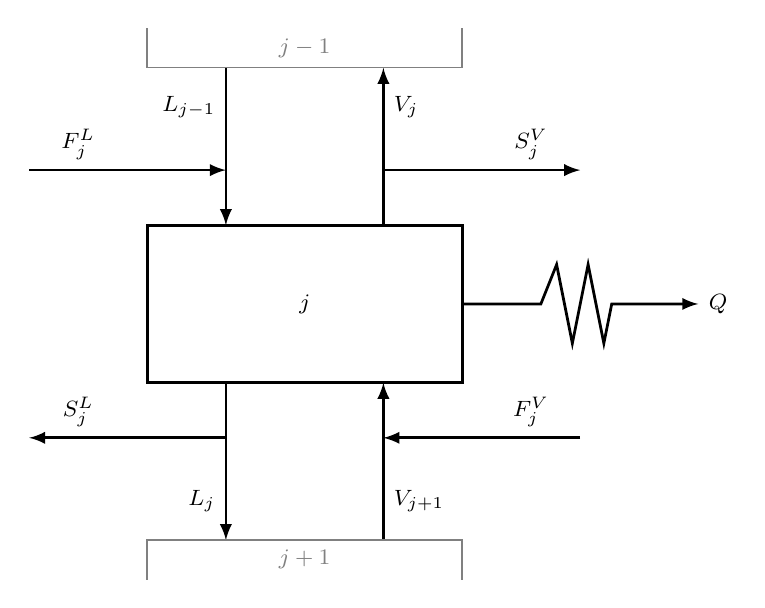
\begin{tikzpicture}[arrow/.style={line width=1pt,->,>=latex}]
	\draw [line width=1pt] (-2,1) rectangle (2,-1) node at (0,0) {\footnotesize $j$};
	\draw [arrow] (-1,3) -- (-1,1) node [pos=0.25, left] {\footnotesize $L_{j-1}$};
 	\draw [arrow] (-3.5,1.7) -- (-1,1.7) node [pos=0.25, above] {\footnotesize $F^L_{j}$};
 	\draw [arrow] (1,1) -- (1,3) node [pos=0.75, right] {\footnotesize $V_{j}$};
 	\draw [arrow] (1,1.7) -- (3.5,1.7) node [pos=0.75, above] {\footnotesize $S^V_{j}$};
 	\draw [arrow] (-1,-1) -- (-1,-3) node [pos=0.75, left] {\footnotesize $L_{j}$};
 	\draw [arrow] (-1,-1.7) -- (-3.5,-1.7) node [pos=0.75, above] {\footnotesize $S^L_{j}$};
	\draw [arrow] (1,-3) -- (1,-1) node [pos=0.25, right] {\footnotesize $V_{j+1}$};
	\draw [arrow] (3.5,-1.7) -- (1,-1.7) node [pos=0.25, above] {\footnotesize $F^V_{j}$};
	\draw [arrow] (2,0) -- (3,0) -- (3.2,0.5) -- (3.4,-0.5) -- (3.6,0.5) -- (3.8,-0.5) -- (3.9,0) -- (5,0,0) node [pos=1, right] {\footnotesize $Q$} ;
    \draw [line width=0.5pt,gray] (-2,-3.5) -- (-2,-3) -- (2,-3) node [pos=0.5, below] {\footnotesize $j+1$} -- (2,-3.5) ; 
    \draw [line width=0.5pt,gray] (-2,3.5) -- (-2,3) -- (2,3) node [pos=0.5, above] {\footnotesize $j-1$} -- (2,3.5) ;
\end{tikzpicture}

            \caption{stage super structure.}
            \label{fig:col_stage_super}
        \end{subfigure}
        %\label{fig:col_super_structs}
        \caption{superstructures for column and column stages.}
    \end{figure}

    \Reffig{fig:col_super} and \reffig{fig:col_stage_super} show the super structures for a distillation column
    with a single feed and and no side draws and an inner column stage.
    The acronym MESH stands for Material (M), Equilibrium (E), Summation (S) and Enthalpy (H)
    equations which are given below.

	\paragraph{Material balances}
        The material balances in their most general form for an inner column stage can be written
        as
        \Eqml{eq:col:CompBalance}{
    		0 = \left(V_j + S_j^V\right) \cdot y_{i,j} + \left(L_j + S_j^L\right) \cdot x_{i,j}
                - V_{j+1} \cdot y_{i,j+1} - L_{j-1} \cdot x_{i,j-1} \\ - F_j^V \cdot z^V_{i,j}
                - F_j^L \cdot z_{i,j}^L, \eqanncs.
    	}%
        \ncr{V_j}{molar vapour flowrate form stage $j$}{\mols}
        \ncr{L_j}{molar liquid flowrate form stage $j$}{\mols}
        \ncr{y_{ij}}{vapour mole fraction of component $i$ on stage $j$}{-}
        \ncr{x_{ij}}{liquid mole fraction of component $i$ on stage $j$}{-}
        \ncr{S^L_j}{molar liquid side-draw flowrate form stage $j$}{\mols}
        \ncr{S^V_j}{molar vapour side-draw flowrate form stage $j$}{\mols}
        \ncr{F^L_j}{molar liquid feed flowrate to stage $j$}{\mols}
        \ncr{F^V_j}{molar vapour feed flowrate to stage $j$}{\mols}
        \ncr{z^L_{ij}}{liquid mole fraction of liquid feed to stage $j$}{-}
        \ncr{z^V_{ij}}{vapour mole fraction of vapour feed to stage $j$}{-}

        Here the vapour and liquid phase of the feed to the stage are considered separately.
        While this is not strictly necessary is allows for certain freedoms in terms of modelling
        column operations, as sometimes the vapour fraction of a given feed is actually fed into
        the vapour phase of a stage and therefore effectively in the liquid phase of the stage above.

        To facilitate convergence the side draw streams $S_j^V$ and $S_j^L$ are made dimensionless
        by means of the respective vapour and liquid flows on that stage to form the
        vapour
        \Eq{eq:val:vap:strip}{
            s_j^V = \frac{S_j^V}{V_j}, \eqanns
        }%
        \ncr{s^V_j}{dimensionless vapour side-draw from stage $j$}{-}
        and liquid
        \Eq{eq:val:vap:strip}{
            s_j^L = \frac{S_j^L}{L_j}, \eqanns
        }%
        \ncr{s^V_j}{dimensionless liquid side-draw from stage $j$}{-}
        stripping factors. Replacing the side-streams in the material balances by their
        corresponding stripping factors yields
        \Eqml{eq:col:CompBalance}{
    		0 = \left(1 + s_j^V\right) \cdot V_j \cdot y_{i,j} + \left(1 + s_j^L\right)
                \cdot L_j \cdot x_{i,j} - V_{j+1} \cdot y_{i,j+1} - L_{j-1} \cdot x_{i,j-1}
                \\ - F_j^V \cdot z^V_{i,j} - F_j^L \cdot z_{i,j}^L,
                \eqannote{i = 1 \dots C, \quad j = 1 \dots N}.
    	}%
        \ncr{C}{number of components}{-}
        \ncr{N}{number of stages}{-}

        As the model is also to be used for optimization purposes further extensions are necessary.
        The location of individual feeds as well as the number of theoretical or real stages of the
        column is to be optimized. To accommodate that need, new variables need, namely the feed
        split $\zeta_{ij}^F$ for feed $i$ to stage $j$ as employed by \cite{Dunnebier.1999} are introduced.
        The split variables are integer variables that can take a value of $0$ or $1$. Additionally it is
        assumed that each feed will only be fed to a single stage thus
        \Eq{eq:col:feedsplit}{
            0 = 1 - \sum_{j=1}^N \zeta_{ij}, \eqannote{i = 1 \dots F, \quad j = 1 \dots N},
        }%
        where $F$ denotes the number of feeds, comprised of vapour ($F^V$) and liquid $F^L$ feeds.

        In order to optimize the number of stages several superstructures are possible. One can
        optimize the reboiler reflux location and condenser reflux location or each single one
        along with the feed and side draw locations. The stage number is then changed as all stages
        between condenser or reboiler reflux are effectively rendered inactive. The solution of
        the mass and energy balances for each respective stages becomes trivial as only one single
        vapour or liquid stream enters and exits the stage. While the choice if condenser and or reboiler
        reflux is optimized is somewhat arbitrary some studies have shown \cite{Grossmann.2005} that
        the strategy of optimizing only feed location and reboiler reflux location possesses some
        numerical advantages in terms of performance of the solution algorithm.

        With the newly introduced split variables for liquid $\zeta^L_{ij}$ and vapour $\zeta^V_{ij}$
        as well as the reboiler reflux $\zeta^R_j$ and the liquid $\zeta^{SL}_{ij}$ and vapour $\zeta^{SV}_{ij}$
        side draws, the material balances can be written as
        \Eqml{eq:col:CompBalance_opt}{
    		0 = \left(1 + s_j^V\right) \cdot V_j \cdot y_{i,j} + \left(1 + s_j^L\right)
                \cdot L_j \cdot x_{i,j} - V_{j+1} \cdot y_{i,j+1} \\ \hfill - L_{j-1} \cdot x_{i,j-1}
                - \sum_{k=1}^{F^V} \zeta_{kj} \cdot F_j^V \cdot z^V_{i,j} - \sum_{l=1}^{F^L}%
                \zeta_{lj} \cdot F_j^L \cdot z_{i,j}^L - \zeta^R_j \cdot V_N \cdot y_{iN}, \hfill%
                \\ \eqannote{i = 1 \dots C, \quad j = 1 \dots N, \quad k = 1 \dots F^V, \quad l = 1 \dots F^L}.
    	}%
        \ncg{\zeta^{L}_{ij}}{splitting variable for liquid feed $i$ on stage $j$}{-}
        \ncg{\zeta^{V}_{ij}}{splitting variable for vapour feed $i$ on stage $j$}{-}
        \ncg{\zeta^{SV}_{ij}}{splitting variable for vapour side draw $i$ on stage $j$}{-}
        \ncg{\zeta^{SL}_{ij}}{splitting variable for liquid side draw $i$ on stage $j$}{-}
        \ncg{\zeta^{R}_{j}}{splitting variable for reboiler reflux on stage $j$}{-}

        Furthermore to be able to optimize side draws, the stripping factors have to be reformulated
        accordingly
        \Eq{eq:val:vap:strip_opt}{
            s_j^V = \frac{\sum_{i=1}^{S^V} \zeta^{SV}_{ij} S_j^V}{V_j}, \eqannote{j = 1 \dots N, \quad i = 1 \dots S^V},
        }%
        \Eq{eq:val:liq:strip_opt}{
            s_j^V = \frac{\sum_{i=1}^{S^L} \zeta^{SL}_{ij} S_j^L}{L_j}, \eqannote{j = 1 \dots N, \quad i = 1 \dots S^L}.
        }%

    \paragraph{Equilibrium equations}
        \todoil{}{add murphee tray efficiency}
        The equilibrium equations are given by
        \Eq{eq:col:Kxy}{
            y_{ij} = K_{ij} \cdot x_{ij}, \eqannote{i = 1 \dots C, \quad j = 1 \dots N}.
    	}%
        \ncr{K_{ij}}{equilibrium ratio of component $i$ on stage $j$}{-}

        Where the equilibrium ratio $K_{ij}$ is computed from the relations that describe
        a vapour liquid equilibrium (VLE).

        A vapour and liquid phase are in equilibrium, when the fugacities in the vapour $f_i^V$
        and liquid $f_i^L$ phase for each species $i$ are equal \cite{AndreasPfennig.2003}
        \Eq{eq:col:fug}{
            f_i^V = f_i^L, \eqannc.
    	}%
        \ncr{f_i^V}{vapour fugacity}{-}
        \ncr{f_i^L}{liquid fugacity}{-}

        This can also be written in terms of the, liquid activity coefficient $\gamma_i$,
        the pointing factor $F_{Pi}$, the reference vapour fugacity coefficient $\varphi_i$,
        the vapour pressure $p^S_i$ as well as the system pressure $p$ along with the vapour and
        liquid molar fractions
        \Eq{eq:col:fug_ext}{
            \gamma_i \, F_{Pi} \, \varphi^0_i \, p^S_i \, x_i = \varphi_i \, p \, y_i, \eqannc.
    	}%
        \ncg{\gamma_i}{liquid activity coefficient of component $i$}{-}
        \ncg{\varphi^0_i}{reference vapour fugacity coefficient of component $i$}{-}
        \ncg{\varphi_i}{vapour fugacity coefficient of component $i$}{-}
        \ncr{p^S_i}{vapour pressure of component $i$}{Pa}
        \ncr{p}{system pressure}{Pa}
        \ncr{F_{Pi}}{compressibility factor of component $i$}{-}

        By reformulating \refeq{eq:col:fug_ext} an expression for the equilibrium ratios
        can be derived
        \Eq{eq:col:fug_ext}{
            y_i = \underbrace{\frac{\gamma_i \, F_{Pi} \, \varphi^0_i \, p^S_i}{\varphi_i \, p}}_{K_i}
                x_i, \eqannc.
    	}%

        The equations to determine the quantities used when computing the equilibrium ratios are by
        themselves functions of temperature, pressure, and vapour as well as liquid molar fractions.
        They are further discussed in \refsec{sec:peng-rob}. It therefore becomes evident that the
        equilibrium ratios are a major source  non-linearities in the MESH equations.

	\paragraph{Enthalpy balances}
        The enthalpy balances can again be written using the previously defined stripping factors
        and splitting variables
    	\Eqml{eq:col:EnergyBalance}{
    		0 = \left(1 + s_j^V\right) \cdot V_j \cdot h^V_{j} + \left(1 + s_j^L\right)
                \cdot L_j \cdot h^L_{j} - V_{j+1} \cdot h^V_{j+1} \\ \hfill - L_{j-1} \cdot h^L_{j-1}
                - \sum_{k=1}^{F^V} \zeta_{kj} \cdot F_k^V \cdot h^{FV}_{j} - \sum_{l=1}^{F^L}
                \zeta_{lj} \cdot F_j^L \cdot h^{FL}_{j} - \zeta^R_j \cdot V_N \cdot h^V_{N}, \hfill
                \\ \eqannote{i = 1 \dots C, \quad j = 1 \dots N, \quad k = 1 \dots F^V, \quad l = 1 \dots F^L}.
    	}%
        \ncr{h^V_j}{molar vapour enthalpy on stage $j$}{\molenth}
        \ncr{h^L_j}{molar liquid enthalpy on stage $j$}{\molenth}
        \ncr{h^{FV}_j}{molar vapour feed enthalpy to stage $j$}{\molenth}
        \ncr{h^{FL}_j}{molar liquid feed enthalpy to stage $j$}{\molenth}

    \paragraph{Condenser and reboiler}
        \begin{figure}
            \centering
            \begin{subfigure}{0.45\textwidth}
                \centering
                \begin{tikzpicture}[scale=0.7]
	\draw [line width=1pt] (-2,1) rectangle (2,-1) node at (0,0) {\footnotesize $1$};
 	\draw [arrow] (1,1) -- (1,3) node [pos=0.75, right] {\footnotesize $V_{1}$};
 	\draw [arrow] (-1,-1) -- (-1,-3) node [pos=0.75, left] {\footnotesize $L_{1}$};
 	\draw [arrow] (-1,-1.7) -- (-3.5,-1.7) node [pos=0.75, above] {\footnotesize $S^L_{1}$};
	\draw [arrow] (1,-3) -- (1,-1) node [pos=0.25, right] {\footnotesize $V_{2}$};
	\draw [arrow] (2,0) -- (3,0) -- (3.2,0.5) -- (3.4,-0.5) -- (3.6,0.5) -- (3.8,-0.5) -- (3.9,0) -- (5,0,0) node [pos=1, right] {\footnotesize $Q^c$} ;
    \draw [line width=0.5pt,gray] (-2,-3.5) -- (-2,-3) -- (2,-3) node [pos=0.5, below] {\footnotesize $2$} -- (2,-3.5) ;
\end{tikzpicture}

                \caption{condenser stage.}
                \label{fig:col_condenser}
            \end{subfigure}
            \begin{subfigure}{0.45\textwidth}
                \centering
                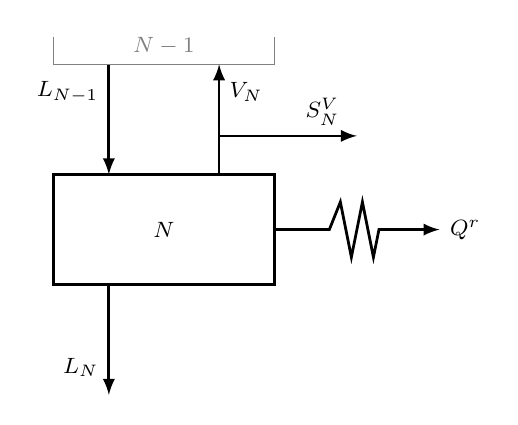
\begin{tikzpicture}[arrow/.style={line width=1pt,->,>=latex},scale=0.7]
	\draw [line width=1pt] (-2,1) rectangle (2,-1) node at (0,0) {\footnotesize $N$};
	\draw [arrow] (-1,3) -- (-1,1) node [pos=0.25, left] {\footnotesize $L_{N-1}$};
 	\draw [arrow] (1,1) -- (1,3) node [pos=0.75, right] {\footnotesize $V_{N}$};
 	\draw [arrow] (1,1.7) -- (3.5,1.7) node [pos=0.75, above] {\footnotesize $S^V_{N}$};
 	\draw [arrow] (-1,-1) -- (-1,-3) node [pos=0.75, left] {\footnotesize $L_{N}$};
	\draw [arrow] (2,0) -- (3,0) -- (3.2,0.5) -- (3.4,-0.5) -- (3.6,0.5) -- (3.8,-0.5) -- (3.9,0) -- (5,0,0) node [pos=1, right] {\footnotesize $Q^r$} ; 
    \draw [line width=0.5pt,gray] (-2,3.5) -- (-2,3) -- (2,3) node [pos=0.5, above] {\footnotesize $N-1$} -- (2,3.5) ;
\end{tikzpicture}

                \caption{reboiler stage.}
                \label{fig:col_reboiler}
            \end{subfigure}
        \end{figure}

        Condenser and reboiler are modeled more or less as regular column stages. However they possess
        certain specialties that are explicitly considered in the column model. For one it is assumed
        that no feeds enter the reboiler and condenser stage. Furthermore no vapour side stream is
        drawn from the condenser stage and no liquid side stream from the reboiler stage.

        Additionally the condenser stage needs to examined a little further. In terms of operations
        several assumptions can be made for the condenser. In general one can distinguish a total,
        partial vapour and partial vapour liquid condenser. For the total condenser all vapour that
        enters the respective stage is condensed and only liquid product is drawn (here modeled as
        a side draw). The partial vapour condenser condenses only the vapour the is fed back into
        the column and all product that is drawn is gaseous. The partial vapour liquid condenser
        denotes the most general case, where part of the incoming vapour is condensed and product
        ist drawn as vapour and liquid. The most important thing to consider in these different cases,
        is that while in both partial condensers a vapour liquid equilibrium takes place, due to the
        absence of vapour the same does not hold for the total condenser. To accommodate that fact
        the MESH equations have to be adjusted \cite{Naphtali.1971}. While the material and energy
        balances remain unchanged the equilibrium equations have to be altered. First the vapour and
        liquid compositions are set equal for all but one component
        \Eq{eq:col:total}{
            x_{i1} = y_{i1} \eqannote{i = 1 \dots C-1},
        }%
        and the condenser temperature is determined by the bubble point equation
        \Eq{eq:col:bub}{
            0 = 1 - \sum_i K_{i1} \cdot x_{i1} \eqannc.
        }%

        When implementing the model in a process simulator it is sensible to consider, that due to
        the limited accuracy of computers the omitted component in \refeq{eq:col:total} needs to
        a non-trace component in the condenser stage. The implemented model therefore as to specify
        such a component when a total condenser is chosen to avoid numerical difficulties.

        In practice it is highly unlikely, that the exact amount of energy required to condensate all
        liquid will be drawn from the condenser. More likely, if all vapour is condensed, a little more
        energy will be withdrawn and slightly sub-cooled liquid will leave the condenser. Therefore
        the model includes the possibility to specify a degree of sub-cooling $T^{sub}$ which will be
        considered when calculating the equilibrium ratios.

    \paragraph{Pressure profile}
        For a steady-state model the pressure profile of a column would usually be specified. However as it
        is inconvenient and unpractical to specify a pressure for each stage one might either specify
        a pressure at the top and bottom stage and assume a uniform pressure profile along the column, or
        specify either top $p_1$ or bottom pressure $p_N$ along with a total pressure drop $\Delta p$,
        or a stage-wise one $\Delta p_{stage}$. However the issue is further complicated if one considers the
        case of optimization for number of trays. In that case several trays will become inactive. For those
        trays the mass and energy balances become trivial, as only liquid enters and exits these trays.
        (For the case employed here, where the reboiler reflux is being optimized). This also means,
        that from the last active tray down to the reboiler -- if present -- there should be a uniform
        profile. however, if a uniform pressure profile from that stage down is not enforced, the solver
        will have to compensate for slight changes in the equilibrium due to pressure variations with minimal
        vapour flow-rates. This is very undesirable, as it might to lead to severe problems in the solver,
        or the calculation of other properties, dependent on these values. To account for this issue, the reboiler
        reflux split can once more be employed
        \Eq{}{
            p_i = p_{j-1} + \left(1 - \sum_{k=1}^{j-1} \zeta^R_k \right) \cdot \Delta p_{j-1} \eqanns.
        }
        \ncr{\Delta p}{pressure drop over entire column}{Pa}
        \ncr{\Delta p_{stage}}{stage-wise pressure drop}{Pa}

        As an alternative to specifying the pressure, one might consider calculating the pressure drop
        form (semi)-empirical models. There a numerous correlations for different types of column internals.
        These correlations become particularly important id column dynamics are to be considered, as they
        make a connection between holdups and flow-rates within the column. Two different pressure drop models
        have been implemented, one for trayed columns and another one for structured packings. As they are closely
        tied to dynamics, they will be discussed in closed detail in \refsec{chp:dynamics}.

    \subsection{Specifications}
        The equation systems presented above is comprised of $NC$ component balances, $NC$ equilibrium
        equations, $2N$ summation equations and $N$ energy balances. This gives a total of $N (2C + 3)$
        equations. On the other hand there are $N$ temperatures and pressures, $2N$ molar flow rates,
        $N$ energy streams, and $NC$ vapour as well as and liquid concentrations. Additionally the feed flow rates
        compositions and temperatures and the side draw split fractions or flow rates appear as variables. The
        feeds and side draws would usually be specified, which leaves a total of $N (2C + 5)$ variables.

        The pressure profile of a distillation column is usually specified. Either by explicitly
        assigning a given pressure to each stage, or more conveniently by defining a pressure
        either the top or bottom pressure as well as the pressure drop per stage
        \Eq{eq:col_pprofile}{
            \Delta p_{stage} = p_i - p_{i-1}, \eqannote{i = 2 \dots N}.
        }
        In terms of unit operations this pressure drop is of high significance,
        as many columns can only be feasibly operated, if the pressure drop does not exceed certain
        limits. In case of the ASU the production of Argon only became feasible as structured
        packings, which display a very low pressure drop, became available. This is due to the large
        number of theoretical stages required to attain the desired Argon purities.

        The energies $Q_i$ denote addition heaters or cooler on the respective stages. For all
        intermediate stages these values would be specified as well. If all energies would be
        specified, that would -- along with the pressure profile -- sum up to $2N$ specifications,
        which leaves $N (2C + 3)$ unknowns. As the number of equations and unknowns are the equal,
        this system can them be solved.

        In practice it is often challenging to correctly guess the condenser and reboiler heat loads in
        advance. This is especially true since they have a tremendous impact on the overall performance
        of the column. Hence it is often desirable to supply other specifications than the respective
        heat loads. To allow for such specification so called discrepancy functions can be introduced \cite{Henley.op.2011},
        which replace the energy balance for the condenser and / or reboiler stage.

        One common specification is the so called reflux ratio $\nu^D = \frac{L_1}{V_1 + S_1^L}$ for
        the condenser, or the boilup ratio $\nu^R = \frac{L_N}{V_N}$ for the reboiler.
        They are defined as the ratio of the molar flowrate sent back into the column over the
        product flowrate which leaves the column. For the reboiler this denotes a liquid stream,
        while for the condenser the product can be gaseous and liquid. Specifying this leads to
        \Eq{eq:reflux}{
            0 & = L_1 - \nu^D \cdot (V_1 + S_1^L), \\
            0 & = V_N - \nu^R \cdot L_N,
        }
        \ncg{\nu^R}{boliup ratio}{-}
        \ncg{\nu^D}{reflux ratio}{-}
        as discrepancy functions. I addition to that further specifications are conceivable. Most
        commonly distillate ($D$) or bottoms ($B$) flow rates, or purities, component flow rates ($d_i, b_i$)
        or temperatures. The corresponding discrepancy functions are summarized in \reftab{tab:discrepancy}.

        \begin{table}
            \centering
            \footnotesize
            \begin{tabular}{lll}
	specification & replacement for $H_1$ & replacement for $H_N$ \\ \hline
	reflux or boilup ratio & $0  = L_1 - \nu^D \cdot (V_1 + S_1^L)$ & $0  = V_N - \nu^R \cdot L_N$ \\
	temperature & $0 = T_1 - T_{spec}$ & $0 = T_N - T_{spec}$ \\
	product flowrate & $0 = (V_1 + S_1^L) - D$ & $0 = L_N - B$ \\
	component product flowrate & & $0 = L_N \cdot x_{iN} - b_i$ \\
	mole fraction & $0 = y_{i1} - y_{i,spec}$ & $0 = x_{iN} - x_{ispec}$ \\ \hline
\end{tabular}

            \caption{discrepancy functions for different column specifications.}
            \label{tab:discrepancy}
        \end{table}

        The specifications for the reboiler stage are quite straightforward, in contrast to that,
        different cases for the condenser have to be considered. In the most general case the
        top product can be drawn as vapour and liquid. This case is here called a partial vapour
        liquid condenser. The other cases are a total condenser, where all the vapour entering the
        condenser stage is condensed, and all product is drawn as a liquid stream, as well as
        a partial vapour condenser, where only the reflux is condensed and all product is drawn
        as vapour. As discussed earlier no VLE takes place in the condenser stage, if a total
        condenser is specified, which needs to be accounted for. Both the total and partial
        vapour condensed implicitly include an extra specification since in former case
        the top vapour product flow rate becomes zero and in the latter the top liquid product
        flowrate. Furthermore a specification of the condenser energy is infeasible as well as implicitly
        given for the total condenser. In case of the partial vapour liquid condenser no implicit
        specification is given, which requires an additional specification. In general two
        top specifications are necessary, whereas only one bottom specification is required.
        These top specification can include the condenser duty, any top flowrate, the reflux ratio
        as well as a newly introduced quantity, the top vapour fraction defined as
        \Eq{}{
            \nu^{vap} = \frac{V_1}{V_1 + S_1^L}.
        }
        \ncg{\nu^{vap}}{condenser vapour fraction}{-}

    \subsection{Column initialization}
        As mentioned before the solution of the MESH equations can pose a considerable problem
        to numerical solvers. It is therefore necessary to supply the solver with feasible
        estimates for the involved variables that can be used as an initial guess to facilitate
        convergence of the process model. A lot of effort has been spend to formulate robust strategies
        to initialize distillation column models. One of the most prominent is the so called
        Inside-Out algorithm first introduced by Boston and Sullivan \cite{Boston.1974}. Within this
        algorithm an inner and outer iterative loop are employed. Within the outer loop approximate
        parameters for simplified models of phase equilibrium and enthalpy are computed by rigorous
        thermodynamic models and guesses for stage temperatures and concentrations. Within the
        inner loop new stage temperatures and concentrations are by solving the MESH equations
        using the simplified thermodynamic models. Once the inner loop converges the simplified
        model parameters are updated within the outer loop by means of the newly calculated
        temperatures and concentrations. This algorithm converges in many cases even for very poor initial
        guesses and has been extended to handle complex columns with side-draws and even reactive
        distillation \cite{BOSTONJ.F..}. It is still in use in the process simulator \aspen.
        However as it is used within an modular algorithmic environment it is not applicable
        to equation based simulators such as \gproms.

        More recently other approaches have been published to attain improved initial guesses.
        Fletcher and Morton \cite{Fletcher.2000} proposed the solution of a column model at
        infinite reflux and zero feed flow rate. This leads to a much simplified model which can
        be solved more easily. The computed purities and stage numbers can give valuable insight
        into the process model. As this approach relies on the solution of a simplified model
        and has no algorithmic elements, it can be implemented in equation based process simulators.

        Another strategy that has been successfully applied to zeotropic and azeotropic mixtures
        relies on solving the column model for the limiting case of the adiabatic column \cite{Barttfeld.2002}.
        The adiabatic column in this case is the column with the minimal entropy production in a real column.
        To avoid entropy production all streams that come in contact must be in equilibrium. To achieve this
        the column would have to employ an infinite number of stages and have an infinite number of
        heat exchangers along its length. The adiabatic column then uses only two heat exchanger in the
        condenser and reboiler stage and assumes a pinch point at the feed stage. \todo{elaborate on adiabatic column}

        Furthermore a much simpler approach has proven adequate for many applications \cite{Henley.op.2011}
        which is also employed as a starting point in this work.
        There feed properties are used as initial guesses. First a linear temperature profile form the boiling
        temperature to dew temperature of the feed is used to initialize temperatures, whereas a simple flash
        at average column pressure and feed temperature yields a vapour and liquid concentration that which is
        used as uniform profile for every column stage. However as the feed might be sub-cooled liquid or
        super-heated vapour the TP-Flash is replaced by a specified vapour fraction. As vapour fraction
        for the flash initial estimates of the vapour and liquid flow rates at the top and bottom of the
        column are used. The stage-wise molar flow-rates are computed from the constant molal overflow
        assumption.

        While this approach leads to model convergence in many cases, it is not entirely robust.
        While the system considered in this case displays only moderate non-idealities it is highly cupeled.
        Especially the low pressure column (LPC) has multiple feeds and side draws, which leads to non-convergence
        if the aforementioned initialization strategy is employed. However the fact that the system is
        not highly non-ideal can be exploited. Whenever the K-values are not too much dependent on mixture
        composition an intermediate step can be used to refine concentration guesses. The constant molal
        overflow assumption is retained and the equilibrium ratios are computed based on the initial guesses
        from the first stage. The component balance is then reformulated only in terms of liquid component
        flow-rates $l_{ij}$

        \Eqml{eq:init:compbalance}{
            0 = \left((1+s_j^V) \cdot K_{ij} \cdot \frac{V_j}{L_j} + (1+s_j^L) \right) \cdot l_{ij}
                - \frac{V_{j+1}}{L_{j+1}} \cdot K_{ij+1} \cdot l_{ij+1} - l_{ij-1}
                \\ - F_j^V \cdot z^V_{i,j} - F_j^L \cdot z_{i,j}^L,
                \eqannote{i = 1 \dots C, \quad j = 1 \dots N}.
        }%
        \ncr{l_{ij}}{liquid molar flowrate of component $i$ from stage $j$}{\mols}
        \ncr{v_{ij}}{vapour molar flowrate of component $i$ from stage $j$}{\mols}

        \refeq{eq:init:compbalance} is linear in the liquid component flow rates. Furthermore vapour component
        flow rates are substituted in the linear component balance and can be computed by

        \Eq{eq:init:vapflow}{
            0 = v_{ij} - K_{ij} \cdot \frac{V_j}{L_j} \cdot l_{ij} \eqannote{i = 1 \dots C, \quad j = 1 \dots N}.
        }%

        On of the reasons \refeq{eq:init:compbalance} is formulated in terms of component flow rates rather
        than molar fractions, is that the molar fraction computed in that manner would not be normalized. If
        the mole fractions are computed from the component flow rates normalization is implicitly given

        \Eq{eq:init:liqmolefrac}{
            x_{ij} = \frac{l_{ij}}{\sum_k^C l_{kj}} \eqannote{i = 1 \dots C, \quad j = 1 \dots N}.
        }%
        \Eq{eq:init:vapmolefrac}{
            y_{ij} = \frac{v_{ij}}{\sum_k^C v_{kj}} \eqannote{i = 1 \dots C, \quad j = 1 \dots N}.
        }%

        The total molar flow rates used in \refeq{eq:init:compbalance} are computed by solving
        stage-wise total mass balances under the constant molal overflow assumption. This assumption
        postulates that the heat of vaporization is independent of system composition.
        Therefore always the same amount of liquid enters and leaves a given stage
    	\Eq{eq:col:cmo}{
    		0 = L_j + S_j^L - L_{j-1} - (1 + q_F^L) \cdot F_j^L - q_F^V \cdot F_j^V
                \eqannote{j = 1 \dots N}.
    	}%
        \ncr{F_j^V}{Vapour feed to tray $j$}{\frac{mol}{s}}
    	\ncr{F_j^L}{Liquid feed to tray $j$}{\frac{mol}{s}}
    	\ncr{S_j^V}{Vapour side flow from tray $j$}{\frac{mol}{s}}
    	\ncr{S_j^L}{Liquid side flow from tray $j$}{\frac{mol}{s}}
    	\ncr{V_j}{Vapour flow from tray $j$}{\frac{mol}{s}}
    	\ncr{L_j}{Liquid flow from tray $j$}{\frac{mol}{s}}

        Only at feed and side draw stages the total flow rates change. To introduce some more accuracy
        to the model, the available information about the feed is considered. When a feed enters as
        super-heated vapour or sub-cooled liquid, it has the capability to evaporate some liquid or
        liquefy some vapour. To account for that fact the feed energy parameters $q_F^L$ and $q_F^V$
        are introduced
        \Eq{eq:feed_en_param}{
            q_i^{FV} & = \frac{H_i^{FV} - H^V_i}{H^V_i - H^L_i}, \eqannote{i = 1 \dots F^V}, \\
            q_i^{FL} & = \frac{H_i^{FL} - H^L_i}{H^V_i - H^L_i}, \eqannote{i = 1 \dots F^L}.
        }

        The vapour total flow rates are then computed from the total mass balances
        \Eq{eq:col:MassBalance}{
    		0 = L_j + S_j^L + V_j + S_j^V - L_{j-1} - V_{j+1} - F_j^L -  F_j^V,
                \eqannote{j = 1 \dots N}.
    	}%

        As no energy balances are included at this stage, the condenser and reboiler stage
        are characterized by the reflux ($\nu^c = \frac{V_1}{L_1}$) or boilup ratio
        ($\nu^r = \frac{V_N}{L_N}$) respectively. This leads to
        \Eq{eq:boilup}{
            0 = V_1 - \nu^c \cdot L_1, \\
            0 = L_N - \nu^r \cdot V_N.
        }

        To close the equation system the global mass balance is included
        \Eq{eq:globalmassbalance}{
            0 = V_1 + L_N + \sum_{j=1}^{N} ( S_j^V + S_j^L - F_j^V - F_j^L ),
                \eqannote{j = 1 \dots N}.
        }
        \subsubsection{Init specification}
            At this point it should be mentioned, that not all specifications are compatible
            with the initialization procedure. As no energy balances are solved during initialization,
            specified condenser or reboiler duties cannot be considered in this stage. Furthermore
            purity specifications are also not applicable during this stage, they are computed by a
            different approach. Due to that it is necessary -- when duties or purities are specified
            -- to supply substitute specifications, that can be used during initialization.
            Essentially all specifications concerning top and bottom flow rates and flow ratios are
            usable during initialization. The user interface implemented specifically asks for
            substitute specifications if any aforementioned cases are encountered.

        \subsubsection{Example}

        \begin{figure}
            \begin{minipage}{0.25\textwidth}
                \begin{tikzpicture}[scale=0.5]
	\draw [line width=0.5pt,gray] (1,4.8) -- (-1,4.8) node [above,pos=0.5,black,yshift=-1mm] {\footnotesize 1};
    \draw [line width=0.5pt,gray] (1,-4.8) -- (-1,-4.8) node [above,pos=0.5,black,yshift=-1mm] {\footnotesize 69};
    \draw [line width=0.5pt,gray] (1,3.2) -- (-1,3.2) node [above,pos=0.5,black,yshift=-1mm] {\footnotesize 10};
    \draw [line width=0.5pt,gray] (1,1.6) -- (-1,1.6) node [above,pos=0.5,black,yshift=-1mm] {\footnotesize 21};
    \draw [line width=0.5pt,gray] (1,0.0) -- (-1,0.0) node [above,pos=0.5,black,yshift=-1mm] {\footnotesize 28};
    \draw [line width=0.5pt,gray] (1,-3.2) -- (-1,-3.2) node [above,pos=0.5,black,yshift=-1mm] {\footnotesize 55};
	\draw [line width=1pt, rounded corners] (-1.0,-5) -- (-1.0,5) .. controls (-0.8,5.8) and (0.8,5.8) .. (1.0,5) node (a) [inner sep=0cm , pos=0.5] {} -- (1.0,-5) .. controls (0.8,-5.8) and (-0.8,-5.8) .. (-1.0,-5) node (b) [inner sep=0cm , pos=0.5] {} -- cycle ; % column tower
    \draw [arrow] (b) -- (0,-6.2) -- (2.5,-6.2) node [draw, line width=1pt, pos=1, circle, minimum size=1.0cm, fill=white] {} -- (2.5,-4.8) -- (1,-4.8) ; % circle reboiler
    \draw [line width=0.5pt] (4,-6.5) -- (2.2,-6.5) -- (2.6,-6.2) -- (2.2,-5.9) -- (4,-5.9) ; % heater reboiler
	\draw [arrow] (-3.0,4.8) -- (-1,4.8) node [above,pos=0.5,black,yshift=-1mm] {\footnotesize $F_1$} ;
    \draw [arrow] (-3.0,1.6) -- (-1,1.6) node [above,pos=0.5,black,yshift=-1mm] {\footnotesize $F_2$} ;
    \draw [arrow] (-3.0,0.0) -- (-1,0.0) node [above,pos=0.5,black,yshift=-1mm] {\footnotesize $F_3$} ;
    \draw [arrow] (-3.0,-3.2) -- (-1,-3.2) node [above,pos=0.5,black,yshift=-1mm] {\footnotesize $F_4$} ;
    \draw [arrow] (1.0,3.2) -- (3.0,3.2) node [above,pos=0.5,black,yshift=-1mm] {\footnotesize $S_1$} ;
    \draw [arrow] (1.0,-3.2) -- (3,-3.2) node [above,pos=0.5,black,yshift=-1mm] {\footnotesize $S_2$} ;
    \draw [arrow] (2.5,-4.8) -- (4,-4.8) ;
    \node at (1.9,-6.2) {\footnotesize 70} ;
    \draw [arrow] (a) -- (0.0,6.5) -- (3.0,6.5) ;
\end{tikzpicture}

                \caption{example column.}
                \label{fig:lpc_example}
            \end{minipage}
            \begin{minipage}{0.73\textwidth}
                \raisebox{\depth}{\footnotesize\begin{tabular}{C{0.08\textwidth}C{0.15\textwidth}C{0.12\textwidth}C{0.12\textwidth}C{0.12\textwidth}C{0.09\textwidth}C{0.09\textwidth}}
    \multicolumn{7}{c}{feed specifications} \\ \hline
	stream & flow $[\frac{kmol}{hr}]$ & $z_{O_2} [-]$ & $z_{N_2} [-]$ & $z_{Ar} [-]$ & $T [K]$ & $p [bar]$ \\ 
	$F_1$ & 2985.77 & 4.674E-10 & 0.9999 & 6.378E-7 & 79.45 & 1.3 \\
	$F_2$ & 1836.36 & 0.2095 & 0.7812 & 0.0093 & 98.91 & 1.3 \\
	$F_3$ & 7609.06 & 0.2920 & 0.6950 & 0.0130 & 81.88 & 1.3 \\
	$F_4$ & 774.94 & 0.9161 & 5.393E-12 & 8.394E-2 & 92.13 & 1.8 \\ \hline 
    & & & & & & \\
    \multicolumn{7}{c}{column specifications} \\ \hline
    stages & $S_1$ frac & $S_2$ frac & \multicolumn{2}{c}{boilup ratio} & $p^{top}$ & $p^{bot}$ \\
    70 & 10 & 0.15 & \multicolumn{2}{c}{3.5} & 1.2 bar & 1.3 bar \\ \hline
\end{tabular}
}
                \captionof{table}{column specifications.}
                \label{fig:lpc_example}
            \end{minipage}
        \end{figure}

        To illustrate how the initialization procedure works an example has been constructed of
        a rather complex column -- or column section -- with multiple feeds and side draws (\reffig{fig:lpc_example}).
        It is taken from an example process of cryogenic air separation. The column in question
        is a column section without an condenser stage and displayed the most difficulties in terms
        of convergence when constructing the process flowsheet.

        In addition to the aforemention initialization strategy, columns with side draws present are handled
        in a slightly different manner. Initially the side draws are disregarded. Then the initialization procedure
        is carried out. Once the column without side draws has converged, a homotopy approach
        \Eq{eq:homotopy}{
            f(\vec{x}) = (1-\alpha) \cdot f_0(\vec{x}) + \alpha \cdot f_1(\vec{x})
        }
        is employed, where the parameter $\alpha$ is initially set to zero and then gradually moved to a value
        of one. \todo{mention problems and bounded homotopy?} During the initialization homotopies could
        generally be employed to move from one step to another. While in some cases robustness is improved by
        such a strategy, it is always computationally far more expensive then simply jumping between different
        stages.

        For clarity reasons the different steps of the initializations procedure a repeated in a tabular manner

        \begin{enumerate}
            \item \cpitemize{
                \item linear temperature profile between dew ($T^{dew}$) and bubble point temperature ($T^{bub}$)
                    of mixed feed.
                \item linear profile between feed flash vapour and liquid compositions for liquid stage
                    compositions.
                \item constant profile for vapour compositions.
                \item molar flow rates from constant molar overflow model.
                \item side draw flow rates set to zero.
            }
            \item \cpitemize{
                \item total molar flow rates form constant molar overflow model.
                \item simplified equilibrium ratios from initial liquid mole fractions and linear
                    temperature profile.
                \item liquid and vapour mole fractions from linearized mass balances.
            }
            \item rigorous solution of MESH equations with side draws still set to zero.
            \item homotopic approach to MESH equations with side draws considered.
        \end{enumerate}

        \ncr{T^{dew}}{dew point temperature}{K}
        \ncr{T^{bub}}{bubble point temperature}{K}

        The resulting profiles for oxygen and nitrogen concentrations in the example column can be seen
        in \reffig{fig:lpc_example_o2} and \reffig{fig:lpc_example_n2}.

        \begin{figure}
            \scriptsize
            \hspace{0.01\textwidth}
            \begin{subfigure}{0.45\textwidth}
                % GNUPLOT: LaTeX picture with Postscript
\begingroup
  \makeatletter
  \providecommand\color[2][]{%
    \GenericError{(gnuplot) \space\space\space\@spaces}{%
      Package color not loaded in conjunction with
      terminal option `colourtext'%
    }{See the gnuplot documentation for explanation.%
    }{Either use 'blacktext' in gnuplot or load the package
      color.sty in LaTeX.}%
    \renewcommand\color[2][]{}%
  }%
  \providecommand\includegraphics[2][]{%
    \GenericError{(gnuplot) \space\space\space\@spaces}{%
      Package graphicx or graphics not loaded%
    }{See the gnuplot documentation for explanation.%
    }{The gnuplot epslatex terminal needs graphicx.sty or graphics.sty.}%
    \renewcommand\includegraphics[2][]{}%
  }%
  \providecommand\rotatebox[2]{#2}%
  \@ifundefined{ifGPcolor}{%
    \newif\ifGPcolor
    \GPcolortrue
  }{}%
  \@ifundefined{ifGPblacktext}{%
    \newif\ifGPblacktext
    \GPblacktexttrue
  }{}%
  % define a \g@addto@macro without @ in the name:
  \let\gplgaddtomacro\g@addto@macro
  % define empty templates for all commands taking text:
  \gdef\gplbacktext{}%
  \gdef\gplfronttext{}%
  \makeatother
  \ifGPblacktext
    % no textcolor at all
    \def\colorrgb#1{}%
    \def\colorgray#1{}%
  \else
    % gray or color?
    \ifGPcolor
      \def\colorrgb#1{\color[rgb]{#1}}%
      \def\colorgray#1{\color[gray]{#1}}%
      \expandafter\def\csname LTw\endcsname{\color{white}}%
      \expandafter\def\csname LTb\endcsname{\color{black}}%
      \expandafter\def\csname LTa\endcsname{\color{black}}%
      \expandafter\def\csname LT0\endcsname{\color[rgb]{1,0,0}}%
      \expandafter\def\csname LT1\endcsname{\color[rgb]{0,1,0}}%
      \expandafter\def\csname LT2\endcsname{\color[rgb]{0,0,1}}%
      \expandafter\def\csname LT3\endcsname{\color[rgb]{1,0,1}}%
      \expandafter\def\csname LT4\endcsname{\color[rgb]{0,1,1}}%
      \expandafter\def\csname LT5\endcsname{\color[rgb]{1,1,0}}%
      \expandafter\def\csname LT6\endcsname{\color[rgb]{0,0,0}}%
      \expandafter\def\csname LT7\endcsname{\color[rgb]{1,0.3,0}}%
      \expandafter\def\csname LT8\endcsname{\color[rgb]{0.5,0.5,0.5}}%
    \else
      % gray
      \def\colorrgb#1{\color{black}}%
      \def\colorgray#1{\color[gray]{#1}}%
      \expandafter\def\csname LTw\endcsname{\color{white}}%
      \expandafter\def\csname LTb\endcsname{\color{black}}%
      \expandafter\def\csname LTa\endcsname{\color{black}}%
      \expandafter\def\csname LT0\endcsname{\color{black}}%
      \expandafter\def\csname LT1\endcsname{\color{black}}%
      \expandafter\def\csname LT2\endcsname{\color{black}}%
      \expandafter\def\csname LT3\endcsname{\color{black}}%
      \expandafter\def\csname LT4\endcsname{\color{black}}%
      \expandafter\def\csname LT5\endcsname{\color{black}}%
      \expandafter\def\csname LT6\endcsname{\color{black}}%
      \expandafter\def\csname LT7\endcsname{\color{black}}%
      \expandafter\def\csname LT8\endcsname{\color{black}}%
    \fi
  \fi
  \setlength{\unitlength}{0.0500bp}%
  \begin{picture}(4762.00,2834.00)%
    \gplgaddtomacro\gplbacktext{%
      \csname LTb\endcsname%
      \put(758,512){\makebox(0,0)[r]{\strut{} 0.0}}%
      \put(758,938){\makebox(0,0)[r]{\strut{} 0.2}}%
      \put(758,1364){\makebox(0,0)[r]{\strut{} 0.4}}%
      \put(758,1789){\makebox(0,0)[r]{\strut{} 0.6}}%
      \put(758,2215){\makebox(0,0)[r]{\strut{} 0.8}}%
      \put(758,2641){\makebox(0,0)[r]{\strut{} 1.0}}%
      \put(1317,352){\makebox(0,0){\strut{} 10}}%
      \put(1831,352){\makebox(0,0){\strut{} 20}}%
      \put(2346,352){\makebox(0,0){\strut{} 30}}%
      \put(2860,352){\makebox(0,0){\strut{} 40}}%
      \put(3374,352){\makebox(0,0){\strut{} 50}}%
      \put(3889,352){\makebox(0,0){\strut{} 60}}%
      \put(4403,352){\makebox(0,0){\strut{} 70}}%
      \put(198,1576){\rotatebox{-270}{\makebox(0,0){\strut{}mole fraction $[-]$}}}%
      \put(2628,112){\makebox(0,0){\strut{}stage number $[\#]$}}%
    }%
    \gplgaddtomacro\gplfronttext{%
      \csname LTb\endcsname%
      \put(3908,1135){\makebox(0,0)[r]{\strut{}step 1}}%
      \csname LTb\endcsname%
      \put(3908,975){\makebox(0,0)[r]{\strut{}step 2}}%
      \csname LTb\endcsname%
      \put(3908,815){\makebox(0,0)[r]{\strut{}step 3}}%
      \csname LTb\endcsname%
      \put(3908,655){\makebox(0,0)[r]{\strut{}conv}}%
    }%
    \gplbacktext
    \put(0,0){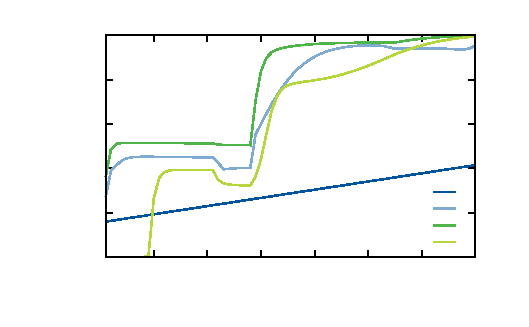
\includegraphics{GNUPlot/LPC_init_o2}}%
    \gplfronttext
  \end{picture}%
\endgroup

                \caption{oxygen concentration profiles.}
                \label{fig:lpc_example_o2}
            \end{subfigure}
            \hfill
            \begin{subfigure}{0.45\textwidth}
                % GNUPLOT: LaTeX picture with Postscript
\begingroup
  \makeatletter
  \providecommand\color[2][]{%
    \GenericError{(gnuplot) \space\space\space\@spaces}{%
      Package color not loaded in conjunction with
      terminal option `colourtext'%
    }{See the gnuplot documentation for explanation.%
    }{Either use 'blacktext' in gnuplot or load the package
      color.sty in LaTeX.}%
    \renewcommand\color[2][]{}%
  }%
  \providecommand\includegraphics[2][]{%
    \GenericError{(gnuplot) \space\space\space\@spaces}{%
      Package graphicx or graphics not loaded%
    }{See the gnuplot documentation for explanation.%
    }{The gnuplot epslatex terminal needs graphicx.sty or graphics.sty.}%
    \renewcommand\includegraphics[2][]{}%
  }%
  \providecommand\rotatebox[2]{#2}%
  \@ifundefined{ifGPcolor}{%
    \newif\ifGPcolor
    \GPcolortrue
  }{}%
  \@ifundefined{ifGPblacktext}{%
    \newif\ifGPblacktext
    \GPblacktexttrue
  }{}%
  % define a \g@addto@macro without @ in the name:
  \let\gplgaddtomacro\g@addto@macro
  % define empty templates for all commands taking text:
  \gdef\gplbacktext{}%
  \gdef\gplfronttext{}%
  \makeatother
  \ifGPblacktext
    % no textcolor at all
    \def\colorrgb#1{}%
    \def\colorgray#1{}%
  \else
    % gray or color?
    \ifGPcolor
      \def\colorrgb#1{\color[rgb]{#1}}%
      \def\colorgray#1{\color[gray]{#1}}%
      \expandafter\def\csname LTw\endcsname{\color{white}}%
      \expandafter\def\csname LTb\endcsname{\color{black}}%
      \expandafter\def\csname LTa\endcsname{\color{black}}%
      \expandafter\def\csname LT0\endcsname{\color[rgb]{1,0,0}}%
      \expandafter\def\csname LT1\endcsname{\color[rgb]{0,1,0}}%
      \expandafter\def\csname LT2\endcsname{\color[rgb]{0,0,1}}%
      \expandafter\def\csname LT3\endcsname{\color[rgb]{1,0,1}}%
      \expandafter\def\csname LT4\endcsname{\color[rgb]{0,1,1}}%
      \expandafter\def\csname LT5\endcsname{\color[rgb]{1,1,0}}%
      \expandafter\def\csname LT6\endcsname{\color[rgb]{0,0,0}}%
      \expandafter\def\csname LT7\endcsname{\color[rgb]{1,0.3,0}}%
      \expandafter\def\csname LT8\endcsname{\color[rgb]{0.5,0.5,0.5}}%
    \else
      % gray
      \def\colorrgb#1{\color{black}}%
      \def\colorgray#1{\color[gray]{#1}}%
      \expandafter\def\csname LTw\endcsname{\color{white}}%
      \expandafter\def\csname LTb\endcsname{\color{black}}%
      \expandafter\def\csname LTa\endcsname{\color{black}}%
      \expandafter\def\csname LT0\endcsname{\color{black}}%
      \expandafter\def\csname LT1\endcsname{\color{black}}%
      \expandafter\def\csname LT2\endcsname{\color{black}}%
      \expandafter\def\csname LT3\endcsname{\color{black}}%
      \expandafter\def\csname LT4\endcsname{\color{black}}%
      \expandafter\def\csname LT5\endcsname{\color{black}}%
      \expandafter\def\csname LT6\endcsname{\color{black}}%
      \expandafter\def\csname LT7\endcsname{\color{black}}%
      \expandafter\def\csname LT8\endcsname{\color{black}}%
    \fi
  \fi
  \setlength{\unitlength}{0.0500bp}%
  \begin{picture}(4762.00,2834.00)%
    \gplgaddtomacro\gplbacktext{%
      \csname LTb\endcsname%
      \put(758,512){\makebox(0,0)[r]{\strut{} 0.0}}%
      \put(758,938){\makebox(0,0)[r]{\strut{} 0.2}}%
      \put(758,1364){\makebox(0,0)[r]{\strut{} 0.4}}%
      \put(758,1789){\makebox(0,0)[r]{\strut{} 0.6}}%
      \put(758,2215){\makebox(0,0)[r]{\strut{} 0.8}}%
      \put(758,2641){\makebox(0,0)[r]{\strut{} 1.0}}%
      \put(1317,352){\makebox(0,0){\strut{} 10}}%
      \put(1831,352){\makebox(0,0){\strut{} 20}}%
      \put(2346,352){\makebox(0,0){\strut{} 30}}%
      \put(2860,352){\makebox(0,0){\strut{} 40}}%
      \put(3374,352){\makebox(0,0){\strut{} 50}}%
      \put(3889,352){\makebox(0,0){\strut{} 60}}%
      \put(4403,352){\makebox(0,0){\strut{} 70}}%
      \put(198,1576){\rotatebox{-270}{\makebox(0,0){\strut{}mole fraction $[-]$}}}%
      \put(2628,112){\makebox(0,0){\strut{}stage number $[\#]$}}%
    }%
    \gplgaddtomacro\gplfronttext{%
      \csname LTb\endcsname%
      \put(3908,1135){\makebox(0,0)[r]{\strut{}step 1}}%
      \csname LTb\endcsname%
      \put(3908,975){\makebox(0,0)[r]{\strut{}step 2}}%
      \csname LTb\endcsname%
      \put(3908,815){\makebox(0,0)[r]{\strut{}step 3}}%
      \csname LTb\endcsname%
      \put(3908,655){\makebox(0,0)[r]{\strut{}conv}}%
    }%
    \gplbacktext
    \put(0,0){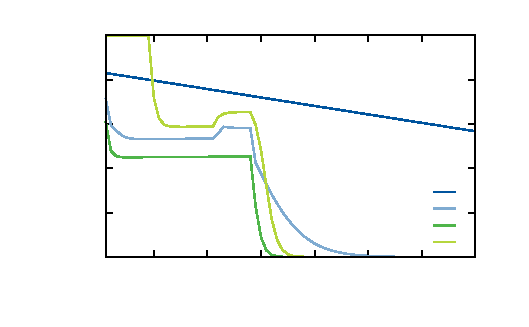
\includegraphics{GNUPlot/LPC_init_n2}}%
    \gplfronttext
  \end{picture}%
\endgroup

                \caption{nitrogen concentration profiles.}
                \label{fig:lpc_example_n2}
            \end{subfigure}
            \hspace{0.01\textwidth}
            \caption{initialization example concentration profiles.}
        \end{figure}

\section{Compression \& liquefaction}
\label{sec:comp_liq}
    The issue of cooling the ambient air to process temperatures at around 90 $K$ is not an easy
    one. The main hindrance is, that a heat sink at this temperature level is not readily available.
    Lucky thermodynamics offer a different way to reach such temperatures. In order to do so,
    the ambient air first needs to be compressed and then expanded again. Cooling then occurs
    by either exploiting the \emph{Joule-Thompson} effect or isentropic expansion. First a few
    comments are made about the compression stage, while afterwards the governing principles
    for cooling by expansion will be described.

    \subsubsection{Multi-stage compression}
        \begin{figure}
            \center
            \begin{tikzpicture}[scale=0.6]
    \compressor{0}{0}{3.0}
    \heater{5}{-2.625}{3}{line width=1pt}
    \draw [line width=1pt] (8,-2.625) -- (8,0) ;
    \compressor{8}{0}{2.0}
    \heater{12}{-2.625}{3}{line width=1pt}
    \draw [line width=1pt] (15,-2.625) -- (15,0) ;
    \compressor{15}{0}{2.0}
    \heater{19}{-2.625}{3}{line width=1pt}
    \draw [arrow] (22,-2.625) -- (23,-2.625) ;
\end{tikzpicture}
            \caption{Multi-stage compression.}
            \label{fig:multi_stage_compression}
        \end{figure}
%        \stdfig{pgfplots/Compressor}{Multi-stage compression.}{fig:multi_stage_compression}{h}

        Compressors and expanders are among the most common process equipment. A multitude of processes
        utilizes them as primary or auxiliary units. While the tasks performed by especially the compressors
        is essential for reaching the required process temperatures, they have less impact in terms of
        process performance and capital expenditure.

        The rigorous modeling of continuous flow machines in terms of unit operations poses great challenges.
        For specific units it may be undertaken by means of CFD simulations or employing characteristics diagrams,
        which require extensive experiments and can usually be obtained from the manufacturer.
        For the purposes of process design however a simpler approach with unit efficiencies is appropriate.

        In order to attain the desired compression it is beneficial, to use a multi stage compressor with
        inter-cooling as depicted in \reffig{fig:multi_stage_compression}. This yields a lower energy consumption
        as a single stage unit for the same compression ratio.

%    	\paragraph{Mass and component balances} The mass and component balances are trivial, as no reactions
%        take place and no phase equilibria have to be considered. It is possible that phase changes might occur
%        within an compressor. While this is certainly relevant during operations of the specific unit, it is not
%        explicitly considered in this model.

%    	\Eq{eq:comp:MassBalance}{
%    		0 = F^{in} - F^{out}
%    	}%
%    	\Eq{eq:comp:CompBalance}{
%    		0 = z_i^{in} - z_i^{out} \eqannote{i = 1 \dots C}
%    	}%
%
%    	\paragraph{Compressor work} To calculate the mechanical work associated with the desired compression,
%        first the isentropic case
%    	\Eq{eq:comp:SInOut}{
%    		S^{in} = S^{out}
%    	}%
%        is considered.
%    	\Eq{eq:comp:IsentropicWork}{
%    		W_S = F^{in} \cdot (H^{in} - H^{out})
%    	}%
%
%    	\paragraph{Compression work}
%    	\Eq{eq:comp:WEta}{
%    		W \cdot \eta^C = W_S
%    	}%
%    	\Eq{eq:comp:CompressionWork}{
%    		W_S = F^{in} \cdot H^{in}(T^{in}, p^{in}, z_i^{in}) - F^{out} \cdot H^{out}(T^{out}, p^{out}, z_i^{out})
%    	}%
%
%    	\paragraph{Pressure drop}
%    	\Eq{eq:comp:PressureDrop}{
%    		p^{out} = p^{in} + \Delta p
%    	}%

    \subsubsection{Cooling by expansion}
        The liquefaction of gases requires temperatures well below ambient conditions. In order to reach
        such conditions one cannot utilize natural occurring coolants, but rather cooling effects that occur
        during the expansion of compressed gases. First we consider the expansion through an expansion valve
        or so called \emph{Joule-Thompson} - valve. If we assume very good insulation of  conditions this
        expansion can closely be approximated by an isenthalpic process ($h_1 = h_2$). To describe the change
        in temperature during isenthalpic expansion the \emph{Joule-Thompson} coefficient
        \Eq{}{
            \mu_{JT} = \left(\fracddpart{T}{p}\right)_h,
        }
        which denotes pressure derivative of the temperature at constant enthalpy can be considered.
        This can be transformed into
        \Eq{}{
            \mu_{JT} = \frac{1}{c_p} \left[T \left(\fracddpart{v}{T}\right)_p - v \right]
        }
        \ncg{\mu_{JT}}{\emph{Joule-Thompson} coeffivcient}{\frac{K}{Pa}}

        \todo{elaborate on different terms.}
        \todo{add derivative in appendix?}

        \begin{figure}
            \center
            % GNUPLOT: LaTeX picture with Postscript
\scriptsize
\begingroup
  \makeatletter
  \providecommand\color[2][]{%
    \GenericError{(gnuplot) \space\space\space\@spaces}{%
      Package color not loaded in conjunction with
      terminal option `colourtext'%
    }{See the gnuplot documentation for explanation.%
    }{Either use 'blacktext' in gnuplot or load the package
      color.sty in LaTeX.}%
    \renewcommand\color[2][]{}%
  }%
  \providecommand\includegraphics[2][]{%
    \GenericError{(gnuplot) \space\space\space\@spaces}{%
      Package graphicx or graphics not loaded%
    }{See the gnuplot documentation for explanation.%
    }{The gnuplot epslatex terminal needs graphicx.sty or graphics.sty.}%
    \renewcommand\includegraphics[2][]{}%
  }%
  \providecommand\rotatebox[2]{#2}%
  \@ifundefined{ifGPcolor}{%
    \newif\ifGPcolor
    \GPcolortrue
  }{}%
  \@ifundefined{ifGPblacktext}{%
    \newif\ifGPblacktext
    \GPblacktexttrue
  }{}%
  % define a \g@addto@macro without @ in the name:
  \let\gplgaddtomacro\g@addto@macro
  % define empty templates for all commands taking text:
  \gdef\gplbacktext{}%
  \gdef\gplfronttext{}%
  \makeatother
  \ifGPblacktext
    % no textcolor at all
    \def\colorrgb#1{}%
    \def\colorgray#1{}%
  \else
    % gray or color?
    \ifGPcolor
      \def\colorrgb#1{\color[rgb]{#1}}%
      \def\colorgray#1{\color[gray]{#1}}%
      \expandafter\def\csname LTw\endcsname{\color{white}}%
      \expandafter\def\csname LTb\endcsname{\color{black}}%
      \expandafter\def\csname LTa\endcsname{\color{black}}%
      \expandafter\def\csname LT0\endcsname{\color[rgb]{1,0,0}}%
      \expandafter\def\csname LT1\endcsname{\color[rgb]{0,1,0}}%
      \expandafter\def\csname LT2\endcsname{\color[rgb]{0,0,1}}%
      \expandafter\def\csname LT3\endcsname{\color[rgb]{1,0,1}}%
      \expandafter\def\csname LT4\endcsname{\color[rgb]{0,1,1}}%
      \expandafter\def\csname LT5\endcsname{\color[rgb]{1,1,0}}%
      \expandafter\def\csname LT6\endcsname{\color[rgb]{0,0,0}}%
      \expandafter\def\csname LT7\endcsname{\color[rgb]{1,0.3,0}}%
      \expandafter\def\csname LT8\endcsname{\color[rgb]{0.5,0.5,0.5}}%
    \else
      % gray
      \def\colorrgb#1{\color{black}}%
      \def\colorgray#1{\color[gray]{#1}}%
      \expandafter\def\csname LTw\endcsname{\color{white}}%
      \expandafter\def\csname LTb\endcsname{\color{black}}%
      \expandafter\def\csname LTa\endcsname{\color{black}}%
      \expandafter\def\csname LT0\endcsname{\color{black}}%
      \expandafter\def\csname LT1\endcsname{\color{black}}%
      \expandafter\def\csname LT2\endcsname{\color{black}}%
      \expandafter\def\csname LT3\endcsname{\color{black}}%
      \expandafter\def\csname LT4\endcsname{\color{black}}%
      \expandafter\def\csname LT5\endcsname{\color{black}}%
      \expandafter\def\csname LT6\endcsname{\color{black}}%
      \expandafter\def\csname LT7\endcsname{\color{black}}%
      \expandafter\def\csname LT8\endcsname{\color{black}}%
    \fi
  \fi
  \setlength{\unitlength}{0.0500bp}%
  \begin{picture}(4762.00,2834.00)%
    \gplgaddtomacro\gplbacktext{%
      \csname LTb\endcsname%
      \put(758,512){\makebox(0,0)[r]{\strut{} 60}}%
      \put(758,816){\makebox(0,0)[r]{\strut{} 70}}%
      \put(758,1120){\makebox(0,0)[r]{\strut{} 80}}%
      \put(758,1424){\makebox(0,0)[r]{\strut{} 90}}%
      \put(758,1729){\makebox(0,0)[r]{\strut{} 100}}%
      \put(758,2033){\makebox(0,0)[r]{\strut{} 110}}%
      \put(758,2337){\makebox(0,0)[r]{\strut{} 120}}%
      \put(758,2641){\makebox(0,0)[r]{\strut{} 130}}%
      \put(1177,352){\makebox(0,0){\strut{} 10}}%
      \put(1535,352){\makebox(0,0){\strut{} 20}}%
      \put(1894,352){\makebox(0,0){\strut{} 30}}%
      \put(2252,352){\makebox(0,0){\strut{} 40}}%
      \put(2611,352){\makebox(0,0){\strut{} 50}}%
      \put(2969,352){\makebox(0,0){\strut{} 60}}%
      \put(3328,352){\makebox(0,0){\strut{} 70}}%
      \put(3686,352){\makebox(0,0){\strut{} 80}}%
      \put(4045,352){\makebox(0,0){\strut{} 90}}%
      \put(4403,352){\makebox(0,0){\strut{} 100}}%
      \put(198,1576){\rotatebox{-270}{\makebox(0,0){\strut{}temperature $[K]$}}}%
      \put(2628,112){\makebox(0,0){\strut{}pressure $[bar]$}}%
    }%
    \gplgaddtomacro\gplfronttext{%
      \csname LTb\endcsname%
      \put(2717,1135){\makebox(0,0)[r]{\strut{}-7000 \sfrac{J}{mol}}}%
      \csname LTb\endcsname%
      \put(2717,975){\makebox(0,0)[r]{\strut{}-6900 \sfrac{J}{mol}}}%
      \csname LTb\endcsname%
      \put(2717,815){\makebox(0,0)[r]{\strut{}-6960 \sfrac{J}{mol}}}%
      \csname LTb\endcsname%
      \put(2717,655){\makebox(0,0)[r]{\strut{}-6850 \sfrac{J}{mol}}}%
    }%
    \gplbacktext
    \put(0,0){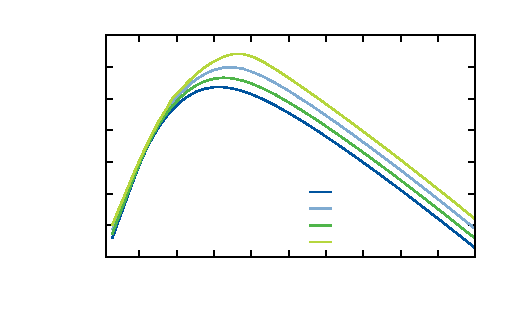
\includegraphics{GNUPlot/pr_isenthalpes}}%
    \gplfronttext
  \end{picture}%
\endgroup

            \caption{Isenthalpes computed by Peng-Robinson EOS.}
            \label{fig:pr_isenthalpes}
        \end{figure}
%        \stdfig{GNUPlot/pr_isenthalpes}{Isenthalpes computed by Peng-Robinson model.}{fig:pr_isenthalpes}{}

        If we employ the Peng-Robinson equation of state we can plot the isenthalpes for ambient air
        ($x_{N_2}=0.7812$, $x_{O_2}=0.2095$, $x_{Ar}=0.0093$ ) in a PT-diagramm (\reffig{fig:pr_isenthalpes}).
        One can easily see, that in certain ranges a pressure decrease will result in an increase in temperature,
        while for other regions in a decrease. It is interesting to mention that the non-idealities
        of a given gas give rise to this effect. For an ideal gas the temperature change at isenthalpic
        expansion would always be zero. Luckily for the cryogenic engineer real gases deviate from ideal
        behaviour especially at elevated pressures and low temperatures. It is therefore important to give some
        consideration to the thermodynamic model used to describe the properties of the system in question, as the
        non-ideal properties need to be captured appropriately.

        A different way of expanding a compressed gas, is by letting it produce work in an fluid kinetic machine.
        If one assumes an adiabatic devices and disregards irreversible effects, this process can be viewed as
        isentropic. Analogous to the isenthalpic case an isentropic expansion coefficient can be defined
        \Eq{}{
            \mu_S = \left( \fracddpart{T}{p} \right)_S = \frac{T}{c_p} \left( \fracddpart{v}{T} \right)_p.
        }%
        \ncg{\mu_S}{isentropic expansion coefficient}{\frac{K}{Pa}}

        Here the derivative in the second form corresponds to the volumetric coefficient of thermal expansion
        $\beta$, which is always positive for gases, which in turn means, that an isentropic expansion
        will always result in an temperature decrease, whereas the isentropic expansion only led to a decrease in
        certain cases. Furthermore an isentropic expansion over the same pressure range will always result in
        lower temperatures than an isenthalpic expansion. Additionally work can be recovered. The reason
        that isentropic valves are most commonly used in liquefaction systems, is that those work producing
        machines cannot handle significant phase changes, which is after all the desired result of liquefaction.

        Traditionally only the isenthalpic expansion had been used within the cryogenic air separation process,
        since -- as mentioned before -- the air needs to be liquefied in order to be fed into be distilled. However
        in modern process configurations the isentropic expansion is also considered, and partial streams are fed into
        the low pressure column in gaseous form.


\section{Heat exchange}
\label{sec:heat_exchange}
    The issue of heat integration is essential to the economic performance of cryogenic air separation. Foremost
    one must consider the special column configuration used in the process. Since operation of the condenser in the
    low pressure section only becomes possible if the reboiler in the high pressure section functions as heat sink,
    no external utilities are supplied to either unit. Rather they are combined into a single heat exchange unit. Thus
    the absolute value of the reboiler energy must matched by the energy recovered from the condenser. Furthermore
    the material streams entering the process can -- and should -- exchange heat with the process streams leaving it.
    The combined condenser / reboiler for LPC / HPC column is assumed as a given heat exchange. This makes sense insofar,
    as this is a necessity in terms of the actual physical implementation of the process units. Also the usage of the
    oxygen rich liquid from the HPC as coolant in the Argon condenser is assumed as fixed.

    This leaves the process stream leaving the compression stage of the process as well as all product and waste streams
    leaving the process. All those streams are -- for simulation purposes and also in some process implementations  -- fed
    into a single multi-stream heat exchange unit. In actual processes all heat exchange and much of the process operations
    take place in the so called ''cold box''. As such a heavily insulated area is referred to. This is done to minimize
    heat exchange with the surroundings. Therefore and for further reasons compact heat exchange units such as plate-fin
    multi-stream heat exchangers are favoured when dealing with cryogenic processes in general and the cryogenic air septation
    in particular.

    Due to the importance of heat integration to the ASU process some thought sould be given as to what modelling approach
    should be employed. Although the field of heat integration is one of the most intensively studied within process engineering,
    only  a limited amount of approaches is available in open literature \cite{Kamath.2012}.

    Traditionally heat integration has been carried out in a sequential manner, where it is for the purposes of process
    optimization assumed, that all heating and cooling is done by external utilities. After an (locally) optimal
    process configuration is identified, all hot and cold streams within the process are identified, and their
    temperature intervals fixed. %In the context of heat integration hot and cold streams do not refer to whether a given
    %stream has a subjectively high or low temperature, but rather whether a given stream needs to be cooled (hot) or
    %heated (cold) within the process. %
    In subsequent steps first the minimum utility requirements, and maximum number of heat exchangers are identified,
    and a specific heat exchange network (HEN) is designed. \todo{add citation Lindhoff...}
    While this approach has been successfully applied to a multitude of processes and led to substantial savings,
    it is questionable if such a sequential approach will yield an optimal or near optimal solution.

    Therefore some efforts have been made to develop efficient strategies for simultaneous process optimization
    and heat integration. Two general approaches can be distinguished. The first one based on the pinch concept.
    \todoil{}{elaborate on pinch concept?} These methods are able to identify the minimum heat requirement
    as well as stream temperatures during process optimization. The first model along these lines was published
    by Duran and Grossmann \cite{Duran.1986} in 1986. They introduced a limited number of quite well behaved
    constraints into the optimization model to ensure no minimum driving force violations. Recently
    this model has been extended to handle phase changes and by fixing the utilities to zero been applied
    to the design of a multi-stream heat exchanger \cite{Kamath.2012}. The major drawback with these methods
    \todoil{}{read about and mention transshipment model by Moriari (sequential)}
    is that one cannot target area of a given heat exchanger as the approach temperatures are not computed
    by the model. Therefore the sometimes substantial trade-off between the cost for heat exchange area
    and utility cost cannot be regarded.

    A second approach employs superstructures of a HEN to find optimal matchings of process streams. No pinch
    point calculations are required, as the actual heat exchange is more or less modeled explicitly. This
    leads to the benefit, that approach temperatures as well as exchanged heat duties between each stream coupling
    are known within the model, and the cost of the designed unit can be considered in an economic objective
    function.

    The approach and respective superstructure adapted in this thesis were first published by Yee and Grossmann
    \cite{Yee.1990}. \Reffig{fig:HX_super} shows the stage wise superstructure for a HEN consisting of two hot
    and two cold streams.

    \begin{figure}
            \begin{tikzpicture}
        \pgfmathsetmacro{\HXsep}{1.5}
        \pgfmathsetmacro{\HXsepup}{1.0}
        \pgfmathsetmacro{\HXrad}{0.5}
        \pgfmathsetmacro{\HXinsep}{0.7}
        \pgfmathsetmacro{\Xsep}{2}
        \pgfmathsetmacro{\Stagesep}{7}
        
        \node (H1_in) [inner sep=0] at (0,0) {} ; 
        \draw ($(H1_in) + (\HXsep,\HXsepup) $) circle (\HXrad) node (HX11) [inner sep=\HXinsep,anchor=center] {\scriptsize $H_1 / C_1$} ; 
        \draw ($(H1_in) + (\HXsep,-\HXsepup) $) circle (\HXrad) node (HX12) [inner sep=\HXinsep,anchor=center] {\scriptsize $H_1 / C_2$} ; 

        \node (H2_in) [inner sep=0] at ($(H1_in) + 3*(0,-\HXsep)$) {} ;
        \draw ($(H2_in) + (\HXsep,\HXsepup) $) circle (\HXrad) node (HX21) [inner sep=\HXinsep,anchor=center] {\scriptsize $H_2 / C_1$} ; 
        \draw ($(H2_in) + (\HXsep,-\HXsepup) $) circle (\HXrad) node (HX22) [inner sep=\HXinsep,anchor=center] {\scriptsize $H_2 / C_2$} ; 
        
        \draw [arrow,RWTHRed] (H1_in) -- (H1_in |- HX11.south west) -- (HX11.south west) ;
        \draw [arrow,RWTHRed] (H1_in) -- (H1_in |- HX12.south west) -- (HX12.south west) ;
        \draw [arrow,RWTHRed] (H2_in) -- (H2_in |- HX21.south west) -- (HX21.south west) ;
        \draw [arrow,RWTHRed] (H2_in) -- (H2_in |- HX22.south west) -- (HX22.south west) ;
        
        \node (H1_in_a) [inner sep=\Xsep] at ($(H1_in) + (-0.5,0)$) {} ;
        \node (H1_in_b) [inner sep=\Xsep] at (H1_in_a |- HX12.north west) {} ;
        \node (H1_in_c) [inner sep=\Xsep] at (H1_in |- HX12.north west) {} ;
        \node (H2_in_b) [inner sep=\Xsep] at (H2_in |- HX22.north west) {} ;
        \node (H2_in_a) [inner sep=\Xsep] at ($(H2_in) + (-1,0)$) {} ;
        
        \draw [arrow,RWTHBlue] (HX21.north west) -- (H1_in_a |- HX21.north west) ;
        \draw [arrow,RWTHBlue] (HX11.north west) -- (H1_in_a |- HX11.north west) ;
        \draw [stdline,RWTHBlue] (H1_in_a |- HX21.north west) -- (H1_in_a |- HX11.north west) ;
        
        \draw [arrow,RWTHBlue] (HX12.north west) -- (H1_in_c) -- (H1_in_b) -- (H2_in_a |- H1_in_b) ;
        \draw [arrow,RWTHBlue] (HX22.north west) -- (H2_in_b) -- (H2_in_b -| H2_in_a) ;
        \draw [stdline,RWTHBlue] (H2_in_b -| H2_in_a) -- (H2_in_a |- H1_in_b) ;
        
        \node (H1_out) [inner sep=0] at ($(H1_in) + (4,0)$) {} ;
        \node (H1_out_a) [inner sep=\Xsep] at ($(H1_out) + (0,-0.5)$) {} ;
        \node (H1_out_b) [inner sep=\Xsep] at ($(HX11.south east) + (1.5,0)$) {} ;
        \node (H1_out_c) [inner sep=\Xsep] at ($(HX12.south east) + (1,0)$) {} ;
        \node (H1_out_d) [inner sep=\Xsep] at (H1_out_b |- H1_out_c) {} ;
        
        \node (H2_out) [inner sep=0] at ($(H2_in) + (4,0)$) {} ;
        \node (H2_out_a) [inner sep=\Xsep] at ($(H2_out) + (0,-0.5)$) {} ;
        \node (H2_out_b) [inner sep=\Xsep] at (H1_out_c |- HX21.south east) {} ;
        \node (H2_out_c) [inner sep=\Xsep] at (H1_out_c |- HX21.north east) {} ;
        
        \draw [arrow,RWTHRed] (HX11.south east) -- (H1_out_b) -- (H1_out_b -| H1_out) ;
        \draw [arrow,RWTHRed] (HX12.south east) -- (H1_out_c) -- (H1_out_d) -- (H1_out_d -| H1_out) ;
        \draw [stdline,RWTHRed] (H1_out_b -| H1_out) -- (H1_out_d -| H1_out) ;
        
        \draw [arrow,RWTHRed] (HX21.south east) -- (H2_out_b) -- (H2_out_b -| H2_out) ;
        \draw [arrow,RWTHRed] (HX22.south east)  -- (HX22.south east -| H2_out) ;
        \draw [stdline,RWTHRed] (H2_out_b -| H2_out) -- (HX22.south east -| H2_out) ;
        
        \draw [arrow,RWTHBlue] (HX22.north east -| H2_out_b) -- (HX22.north east) ;
        \draw [arrow,RWTHBlue] (HX12.north east -| H2_out_b) -- (HX12.north east) ;
        \draw [stdline,RWTHBlue] (HX12.north east -| H2_out_b) -- (HX22.north east -| H2_out_b) ;
        
        \draw [arrow,RWTHBlue] (HX21.north east -| H1_out_d) -- (H2_out_c) -- (HX21.north east) ; 
        \draw [arrow,RWTHBlue] (HX11.north east -| H1_out_b) -- (HX11.north east) ;
        \draw [stdline,RWTHBlue] (HX11.north east -| H1_out_b) -- (HX21.north east -| H1_out_d) ;
        
        \node (H1_mid) [inner sep=0] at ($(H1_in) + (\Stagesep,0)$) {} ; 
        \draw ($(H1_mid) + (\HXsep,\HXsepup) $) circle (\HXrad) node (HX31) [inner sep=\HXinsep,anchor=center] {\scriptsize $H_1 / C_1$} ; 
        \draw ($(H1_mid) + (\HXsep,-\HXsepup) $) circle (\HXrad) node (HX32) [inner sep=\HXinsep,anchor=center] {\scriptsize $H_1 / C_2$} ; 

        \node (H2_mid) [inner sep=0] at ($(H1_mid) + 3*(0,-\HXsep)$) {} ;
        \draw ($(H2_mid) + (\HXsep,\HXsepup) $) circle (\HXrad) node (HX41) [inner sep=\HXinsep,anchor=center] {\scriptsize $H_2 / C_1$} ; 
        \draw ($(H2_mid) + (\HXsep,-\HXsepup) $) circle (\HXrad) node (HX42) [inner sep=\HXinsep,anchor=center] {\scriptsize $H_2 / C_2$} ; 
        
        \draw [arrow,RWTHRed] (H1_mid) -- (H1_mid |- HX31.south west) -- (HX31.south west) ;
        \draw [arrow,RWTHRed] (H1_mid) -- (H1_mid |- HX32.south west) -- (HX32.south west) ;
        \draw [arrow,RWTHRed] (H2_mid) -- (H2_mid |- HX41.south west) -- (HX41.south west) ;
        \draw [arrow,RWTHRed] (H2_mid) -- (H2_mid |- HX42.south west) -- (HX42.south west) ;
        
        \node (H1_mid_a) [inner sep=\Xsep] at ($(H1_mid) + (-0.5,0)$) {} ;
        \node (H1_mid_b) [inner sep=\Xsep] at (H1_mid_a |- HX32.north west) {} ;
        \node (H1_mid_c) [inner sep=\Xsep] at (H1_mid |- HX32.north west) {} ;
        \node (H2_mid_b) [inner sep=\Xsep] at (H2_mid |- HX42.north west) {} ;
        \node (H2_mid_a) [inner sep=\Xsep] at ($(H2_mid) + (-1,0)$) {} ;
        
        \draw [arrow,RWTHBlue] (HX41.north west) -- (H1_mid_a |- HX41.north west) ;
        \draw [arrow,RWTHBlue] (HX31.north west) -- (H1_mid_a |- HX31.north west) ;
        \draw [stdline,RWTHBlue] (H1_mid_a |- HX41.north west) -- (H1_mid_a |- HX31.north west) ;
        
        \draw [arrow,RWTHBlue] (HX32.north west) -- (H1_mid_c) -- (H1_mid_b) -- (H2_mid_a |- H1_mid_b) ;
        \draw [arrow,RWTHBlue] (HX42.north west) -- (H2_mid_b) -- (H2_mid_b -| H2_mid_a) ;
        \draw [stdline,RWTHBlue] (H2_mid_b -| H2_mid_a) -- (H2_mid_a |- H1_mid_b) ;
        
        \node (H3_out) [inner sep=0] at ($(H1_mid) + (4,0)$) {} ;
        \node (H3_out_a) [inner sep=\Xsep] at ($(H3_out) + (0,0.5)$) {} ;
        \node (H3_out_b) [inner sep=\Xsep] at ($(HX31.south east) + (1.5,0)$) {} ;
        \node (H3_out_c) [inner sep=\Xsep] at ($(HX32.south east) + (1,0)$) {} ;
        \node (H3_out_d) [inner sep=\Xsep] at (H3_out_b |- H3_out_c) {} ;
        
        \node (H4_out) [inner sep=0] at ($(H2_mid) + (4,0)$) {} ;
        \node (H4_out_a) [inner sep=\Xsep] at ($(H4_out) + (0,0.5)$) {} ;
        \node (H4_out_b) [inner sep=\Xsep] at (H3_out_c |- HX41.south east) {} ;
        \node (H4_out_c) [inner sep=\Xsep] at (H3_out_c |- HX41.north east) {} ;
        
        \draw [arrow,RWTHRed] (HX31.south east) -- (H3_out_b) -- (H3_out_b -| H3_out) ;
        \draw [arrow,RWTHRed] (HX32.south east) -- (H3_out_c) -- (H3_out_d) -- (H3_out_d -| H3_out) ;
        \draw [stdline,RWTHRed] (H3_out_b -| H3_out) -- (H3_out_d -| H3_out) ;
        
        \draw [arrow,RWTHRed] (HX41.south east) -- (H4_out_b) -- (H4_out_b -| H4_out) ;
        \draw [arrow,RWTHRed] (HX42.south east)  -- (HX42.south east -| H4_out) ;
        \draw [stdline,RWTHRed] (H4_out_b -| H4_out) -- (HX42.south east -| H4_out) ;
        
        \draw [arrow,RWTHBlue] (HX42.north east -| H4_out_b) -- (HX42.north east) ;
        \draw [arrow,RWTHBlue] (HX32.north east -| H4_out_b) -- (HX32.north east) ;
        \draw [stdline,RWTHBlue] (HX32.north east -| H4_out_b) -- (HX42.north east -| H4_out_b) ;
        
        \draw [arrow,RWTHBlue] (HX41.north east -| H3_out_d) -- (H4_out_c) -- (HX41.north east) ; 
        \draw [arrow,RWTHBlue] (HX31.north east -| H3_out_b) -- (HX31.north east) ;
        \draw [stdline,RWTHBlue] (HX31.north east -| H3_out_b) -- (HX41.north east -| H3_out_d) ;
        
        \draw [arrow,RWTHRed] ($(H1_in) + (-2.5,0)$) node [left,black] {\footnotesize $H_1$} -- (H1_in_a) -- (H1_in) ;
        \draw [arrow,RWTHRed] ($(H2_in) + (-2.5,0)$) node [left,black] {\footnotesize $H_2$} -- (H2_in_a) -- (H2_in) ;
        \draw [arrow,RWTHBlue] ($(H1_in) + (-0.5,0.5)$) -- ($(H1_in) + (-2.5,0.5)$) node [left,black] {\footnotesize $C_1$} ;
        \draw [arrow,RWTHBlue] ($(H2_in) + (-1,0.5)$) -- ($(H2_in) + (-2.5,0.5)$) node [left,black] {\footnotesize $C_2$} ;
        
        \draw [arrow,RWTHRed] (H1_out) -- (H1_mid_a) -- (H1_mid) ;
        \draw [arrow,RWTHRed] (H2_out) -- (H2_mid_a) -- (H2_mid) ;
        \draw [arrow,RWTHBlue] (H2_mid_a |- H2_out_a) -- (H2_out_a) -- ++(-1,0) ;
        \draw [arrow,RWTHBlue] (H1_mid_a |- H1_out_a) -- (H1_out_a) -- ++(-0.5,0) ;
        
        \draw [arrow,RWTHBlue] ($(H3_out_a) + (1.5,-1)$) node [right,black] {\footnotesize $C_1$} -- ($(H3_out_a) + (0,-1)$) -- ++(-0.5,0) ;
        \draw [arrow,RWTHBlue] ($(H4_out_a) + (1.5,-1)$) node [right,black] {\footnotesize $C_2$} -- ($(H4_out_a) + (0,-1)$) -- ++(-1,0) ;
        \draw [arrow,RWTHRed] ($(H3_out_a) + (0,-0.5)$) -- ++(1.5,0) node [right,black] {\footnotesize $H_1$} ; 
        \draw [arrow,RWTHRed] ($(H4_out_a) + (0,-0.5)$) -- ++(1.5,0) node [right,black] {\footnotesize $H_2$} ; 
        
        \draw[dashvol] (-2,2) -- (-2,-7) ;
        \draw[dashvol] ($(-2,2) + (\Stagesep,0)$) -- ($(-2,-7) + (\Stagesep,0)$) ;
        \draw[dashvol] ($(-2,2) + 2*(\Stagesep,0)$) -- ($(-2,-7) + 2*(\Stagesep,0)$) ;
        
        \node at (-2,-7.3) {\footnotesize $\ell = 1$} ;
        \node at ($(-2,-7.3) + (\Stagesep,0)$) {\footnotesize $\ell = 2$} ; 
        \node at ($(-2,-7.3) + 2*(\Stagesep,0)$) {\footnotesize $\ell = 3$} ;
        
        \node at ($(HX11) + (0,1.5)$) {Stage 1} ; 
        \node at ($(HX31) + (0,1.5)$) {Stage 2} ;
        
    \end{tikzpicture}

        \caption{Superstructure for multi-stream heat exchanger. \cite{Yee.1990}}
        \label{fig:HX_super}
    \end{figure}
%    \stdfig{Pictures/HX_superstructure}{Superstructure for multi-stream heat exchanger. \cite{Yee.1990}}{fig:HX_super}{}

    In this stagewise structure each hot stream can exchange heat with each cold stream within each stage.
    The following assumptions were made when the model was developed
    \begin{itemize}
        \item Constant heat capacities
        \item Constant heat transfer coefficients
        \item Countercurrent heat exchangers
        \item Isothermal mixing at each stage.
    \end{itemize}

    The assumption of constant heat capacities is a common one in the design of HEN's. When no phase boundaries are passed
    and the temperature range of the involved is not too wide, it is a reasonably good approximation of the real conditions.
    While constant heat transfer coefficients a re assumed the model leaves the flexibility to define different
    coefficients for each pairing of hot and cold streams. Countercurrent heat exchangers are common in industrial practice.
    This assumption however does not really pose a limitation, as the model can easily be altered to account for concurrent
    units.

    The last assumption of isothermal mixing is a more major one. It has been introduced as it allows for significant
    simplifications and leads to a model, where all constraints are linear and all non-linearities are restricted
    to the objective function. While that is certainly not true for the entire process model, it should at least
    allow for some reductions in the model complexity. The assumption states, that regardless of which streams a
    given stream exchanges heat with, it will leave at the same temperature. Due to that all energy balances around
    each unit in the superstructure can be eliminated as well as the subsequent mixing of the streams.

    \paragraph{Model equations}

    First of all a heat balance at each stage is necessary
    \Eq{}{
        F_i (T_{i, \ell} - T_{i, \ell+1}) = \sum_j q_{ijk} \\
        f_j (T_{i, \ell} - T_{i, \ell+1}) = \sum_i q_{ijk}
    }

    The heat exchange area $A_{hx}$ can be computed from the exchanged energy, the heat transfer coefficients $\alpha_{ij}$
    and the logarithmic mean temperature difference $LMTD$.
    \Eq{}{
        A_{hx} = \sum_i \sum_j \sum_k \frac{q_{ijk}}{\alpha_{ij} * LMDT_{ijk} + \delta}
    }

    While the small number $\delta$ is included to avoid problems in the program, when $LMDT$ becomes zero
    In order to avoid further numerical difficulties when the approach temperatures $\Delta T_{ij}$ at each side of an exchange
    unit approach zero, it was proposed to use an approximation introduced by Chen \cite{Chen.1987}
    \Eq{}{
        LMDT_{ijk} \approx \left[ \Delta T_{ijk} \cdot \Delta T_{ijk+1} \frac{\Delta T_{ijk} + \Delta T_{ijk+1}}{2} \right]^{\frac{1}{3}}.
    }

    While the approach temperatures are defined as
    \Eq{}{
        \Delta T_{ijk} = \max \left\{0, T_{ik} - T_{jk}\right\}
    }
    AS the $\max$ function is non-smooth and thus non differentiable at the points $T_{ik} = T_{jk}$, \gproms internally uses a smooth
    approximation. The exact for of which is unknown to the author.

\section{Integrated condenser reboiler unit}

%\subsection{Centrifugal pump}
%	
%	\paragraph{Cost estimation}
%		The cost for the pump excluding the motor can be approximated by
%		\Eq{eq:pump:CostPump}{
%			C_B & = \exp \left[ 9.7171 - 0.6019 \ln[S] + 0.0519 (\ln[S])^2 \right] \eqannote{40 \leq S \leq 100000}\\
%			C_p & = f_T \, f_M \, C_B.
%		}
%		The cost for the centrifugal pump is approximated by the value $S = Q \cdot \sqrt{H} $, where
%		$Q$ denotes the volume flow through the pump in gallons per minute $[gpm]$ and $H$ the
%		pump head in $[ft]$.
%		
%		The costs given above is excluding the motor needed. It is then estimated separately. In this
%		case the specific quantity is the power consumption $P_C$ needed for the desired stream transport.
%		
%		\Eqml{eq:pump:CostMotor}{
%			C_B  = \exp\big[ 5.8259 + 0.13141 \ln[P_C] + 0.053255 (\ln[Pc])^2 \\
%				 + 0.028628 (\ln[P_C])^3 - 0.0035549 (\ln[P_C])^4 \big]
%		}	


%\subsubsection{Expander}


%\subsection{Heater}
%
%	\stdfig{pgfplots/Heater}{Heater model.}{fig:Heater}{h}
%
%	\paragraph{Mass and component balances}
%	\Eq{eq:comp:MassBalance}{
%		0 = F^{in} - F^{out}
%	}%
%	\Eq{eq:comp:CompBalance}{
%		0 = z_i^{in} - z_i^{out}
%	}%
%	
%	\paragraph{Pressure drop}
%	\Eq{eq:reboil:PressureDrop}{
%		p^R = p^{in} + \Delta p
%	}%
%	
%	\todo[inline]{add formulas for vapour fraction}
%		
%\subsubsection{Pump}
%
%\subsubsection{Separator}
%
%\subsubsection{Joule-Thompson valve}
%    \todo{add effect for cooling....}
%
%\subsection{Splitter}
%	\stdfig{pgfplots/Splitter}{Splitter model}{fig:Splitter}{h}
%	The splitter is a fairly simple process component. Its sole purpose is -- as the name
%    suggests -- to split a given material stream into several sub-streams. No reactions
%    or heat exchange take place in this unit. The molar properties remain unchanged.
%    The global mass balance is therefore the governing equation for this unit where
%    the feed $F^{in}$ is split according to the split fractions $\xi_i$ into $N^s$
%    sub-streams
%	\paragraph{Mass and component balances}
%	\Eq{eq:comp:MassBalance}{
%        0 = F_i^{out} - F^{in} \cdot \xi_i, \eqannote{i = 1 \dots }, \\
%        0 = 1 - \sum_{i=1}^{N^s}
%	}%
%
%    \paragraph{Pressure drop}
%    To take into account the actual unit a pressure drop over the unit can be specified
%	\Eq{eq:split:PressureDrop}{
%		p^{out} = p^{in} + \Delta p.
%	}%

\section{Thermodynamic models}
\label{sec:peng-rob}
    Aside from the unit operation models, the behaviour of materials in a process needs to be adequately
    accounted for. This is done by means of so called equations of state (EOS) and excess Gibbs energy
    models. In terms of thermodynamics there are only a limited amount of variables. Namely the pressure,
    density and temperature as well as composition. While equations of state can model a given system in
    the vapour as well as liquid phase, excess Gibbs energy models only account for the behaviour of a liquid
    and need to be used in conjunction with other models for the vapour phase. However they have shown
    considerable better performance for highly non-ideal systems \cite{AndreasPfennig.2003}. As mentioned
    earlier (\refsec{sec:comp_liq}) it is essential to accurately capture the non-idealities of air
    in order to capture the liquefaction process. In the case of cryogenic air separation, the Peng-Robinson
    as well as the Benders equation of state have shown satisfactory performance. The Peng-Robinson equation
    was chosen to be used in the presented model
    \Eq{eq:peng_rob}{
        p & = \frac{RT}{V-b} - \frac{a_c \left[1+m\left(1-\sqrt{T_r}\right)\right]^2}{V^2+2bV-b^2} \\
        m & = 0.37464 + 1.54226 \omega - 0.26992 \omega^2 \\
        a_c & = 0.45724 \frac{R^2T_c^2}{p_c} \\
        b & = 0.077796 \frac{RT_c}{p_c} \\
        \omega & = -1 - \log_{10} \, (p_r^{sat})_{T_r = 0.7}
    }
    \ncr{p}{pressure}{Pa}
    \ncr{m}{parameter in Peng-Robinson EOS}{-}
    \ncr{a_c}{parameter in Peng-Robinson EOS}{\frac{m^5}{mol^2 s^2}}
    \ncr{b}{parameter in Peng-Robinson EOS}{\frac{m^3}{mol}}
    However the Peng-Robinson EOS relies on the so called one-fluid theory which models each fluid as pure.
    To model mixtures the pure component parameters have to be ''mixed''
    \Eq{}{
        a & = \sum_{i=1}^C \sum_{j=1}^C y_i y_j a_{ij}, \\
        a_{ij} & = \sqrt{a_i a_j} (1 - k_{ij}), \\
        b & = \sum_{i=1}^C y_i b_i.
    }

    From that EOS numerous relevant properties such as excess enthalpy, fugacity coefficients or densities
    can be calculated. For a list of some relevant equations refer to \refsec{app:peng_rob_deriv}.
    \todo{which properties should be included? Or move everything to Appendix?}
	
\section{Economic models}
\label{sec:EconModel}
	As discussed earlier economic consideration play a major role in process design. In order to account
	for the process economics the cost of the process to be implemented needs to be estimated at the design
	level. However as limited information is available estimation methods have to be employed. In
	\refsec{chp:ProcesEconomics} the general approach for cost estimation of process equipment was
	introduced, where a specific value such as heat-exchange area or vessel size is used to approximate
	equipment cost. However for more specific units extended models are available, where statistical
	data is employed to yield a more realistic fit to cost data. The cost functions and correction
	factors presented in this chapter are, if not stated otherwise, taken from \cite{Seider.2010}.
	Also unless otherwise stated the unit cost is given for the year 2006 ($CE = 500$).
	
	\subsubsection{Destillation column}
		Out of all the process equipment the distillation column probably is the most elaborate
		unit. It also poses the greatest challenges when it comes to finding an appropriate
		estimate for its cost. This is die to the fact that the column in itself is rather
		large and complex. To properly operate a column the vessel needs to have numerous
		valves, scaffolding and several manholes. Due to its size further factors come into
		play that need not to be considered for the other relatively small units. Those location
		dependent factors might include resilience towards earthquakes, the ability to withstand
		close winds or intensive ambient temperatures. However as the scope of this work explicitly
		focuses on early design stages those location specific influences will be disregarded
		to arrive at simpler models for cost estimation.
		
		\paragraph{Vertical tower}
			The cost for the vessel $C_V$ which is to be vertically erected vertically is dependent
			on teh weight fo the weight $W$ ($[lbs]$) of the vessel. This includes valves, manholes and
			other details directly connected with the tower. However the cost for ladders,
			platforms and railings necessary to properly operate the column are calculated
			separately
			\Eq{eq:cost:column:column}{
				C_p = f_M \, C_V + C_{PL}.
			}
			
			The correlated equation for the cost of the tower is given by
			\Eq{eq:cost:column:vessel}{
				C_V = \exp\big\{ 7.2756 + 0.18255 \cdot \ln[W] + 0.02297 \cdot \pow{\ln[W]}{2} \big\}, \eqannote{9000 \leq W \leq 2.5 \cdot 10^6}.
			}
			
			To the cost of the tower, the cost of the surrounding support structure ist added. It is dependent
			on the inner diameter of the vessel ($D_i$) as well as the so called tangent to tangent length ($L$).
			This denotes the length of the tube that makes up the vessel excluding the spherical domes that
			close the column on each side. With that the additional cost is then computed by
			\Eq{eq:cost:column:support}{
				C_{PL} = 300.9 \cdot \pow{D_i}{0.63316} \cdot \pow{L}{0.80161}.
			}
			
		\paragraph{Weight}
			As can be seen from the above correlations the weight of the column is a determining factor
			for the estimated and actual cost. Therefore some thought should be put into how this can
			be determined, when the final design is unknown. Again several correlations have been applied
			to real life units which yield satisfactory results. In general the weight of the empty vessel
			can be computed by determining the volume of the material and multiplying it with its density ($\varrho$)
			\Eq{eq:cost:column:weight}{
				W = \pi (D_i + t_s)(L + 0.8 \cdot D_i) t_s \cdot \varrho.
			}
			The term $0.8 D_i$ is included to approximate the weight of the domes, whereas $t_s$ is the shell
			thickness. To determine how thick the walls of the shell need to be the ASME pressure vessel code
			formula is often applied
			\Eq{eq:cost:column:wallthickness}{
				t_s = \frac{P_d \, D_i}{2 \, S \, E - 1.2 P_d}.
			}
			Where the maximal allowable stress $S$, which the chosen material can withstand at
			process conditions is multiplied by the fractional weld efficiency $E$ to regard the effects
			of the manufacturing process on the material strength. To ensure an error on the side of
			caution the design pressure $P_d$ is calculated from the actual operating pressure $P_o$
			by means of
			\Eq{eq:cost:column:designpressure}{
				P_d = \exp\big\{ 0.60600 + 0.91615 \cdot \pow{\ln[P_o]}{} + 0.0015655 \cdot \pow{\ln[P_o]}{2}
			}
			It is important to consider, that the maximum allowable stress especially needs to take into account
			the operating temperature of the distillation process, as it might have significant effects.
			
			Furthermore the given formulas only apply to pressures above ambient conditions. Thus low pressure
			or vacuum distillation is not covered by the presented formulas.
			
		\paragraph{Column internals}
			While internal support structures are already considered by the equations given above, the
			internals responsible to ensure product separation are not. Those make up a very significant
			amount of the total column cost and are available .
	       \todo{finish column internals}

	\subsubsection{Centrifugal pump}
		Pumps are among the most common units of process equipment. While there are several different
		kinds of pumps that can be used, the centrifugal pump is one of the most popular choices and
		denotes a very likely choice for the process conditions considered in this application. Hence
		other pump types will not be considered at this point.
		
		\paragraph{Pump}
			In terms of operations pumps are best described by the volumetric flow transported $Q$ as
			well as the pump head $H$, the hight that needs to be overcome. Data taken from the company
			Mosanto was used to correlate the pump cost to a specific value
			\Eq{eq:cost:pump:SpecVal}{
				S = Q \sqrt{H}.
			}
			As a reference unit the base price $C_B$ is estimated for a cast iron single-stage
			vertically split case at 3600 $rpm$
			\Eq{eq:cost:pump:PumpWOMotor}{
				C_B = \exp \left\{ 9.7171 - 0.6019 \cdot \ln[S] + 0.0519 (\ln[S])^2 \right\},
					\eqannote{400 \leq S \leq 100000}.
			}
			
			The most influential addition factors for the pump price are the material, which is accounted
			for in the material factor $f_m$, as well as the rotation, case split orientation (horizontal
			and vertical), the number of stages, covered flow rate range, pump head range and maximum
			motor power, which are all agglomerated in the type factor $f_T$. Values for these factors
			are given in \reftab{tab:pump:Type} and \reftab{tab:pump:Material}.
			
			\stdtab{Tables/PumpFactorsType}{Pump type factors \cite{Seider.2010}.}{tab:pump:Type}
			\stdtab{Tables/PumpFactorsMaterial}{Pump material factors \cite{Seider.2010}.}{tab:pump:Material}
			
		\paragraph{Electric motor}
			Separately from the pump itself the motor to drive the compression is considered. While the
			volumetric flow and the pump head certainly are valid choices to correlate motors for pumps
			especially, the power consumption is a more general specific value
			\Eq{eq:cost:pump:MotorPowerConsumption}{
				P_C = \frac{P_T}{\eta_P \eta_M} = \frac{P_B}{\eta_M}
			}
			
			It can be calculated from the theoretic power of the pump $P_T$ and the efficiencies $\eta_P$
			$\eta_M$. While an estimate for the expected power consumption might be already available at
			rather early design stages, the efficiencies will have to be correlated as well if resorting
			to average values is considered too coarse. Those correlations rely on the volumetric flow in
			gallons per minute ([gpm]) and the brake horse power $P_B = \frac{P_T}{\eta_P}$.
			
			\Eq{eq:cost:pump:MotorEfficiancyP}{
				\eta_P = -0.316 + 0.24015 \cdot \ln[Q] - 0.01199 \cdot (\ln[Q])^2 \eqannote{50 \leq Q \leq 5000}
			}
			\Eq{eq:cost:pump:MotorEfficiancyM}{
				\eta_M = 0.80 + 0.0319 \cdot \ln[P_B] - 0.00182 \cdot (\ln[P_B])^2 \eqannote{1 \leq P_B \leq 1500}
			}
			
			After having calculated the power which the motor needs to supply its base cost of an open,
			drip-proof enclosed motor at 3600 $rpm$ can be approximated by
			\Eqml{eq:cost:pump:Motor}{
				C_B = \exp\big\{ 5.8259 + 0.13141 \cdot \ln[P_C] + 0.053255 \cdot (\ln[P_C])^2 \\
					+ 0.028628 \cdot (\ln[P_C])^3 - 0.0035549 \cdot (\ln[P_C])^4 \big\} \eqannote{1 \leq P_C \leq 700}
			}
			
			To adjust the cost for different types of electric motors the type factors from \reftab{tab:pump:MotorTypes}
			
			\stdtab{Tables/MotorTypeFactors}{Type factors for different motor types.}{tab:pump:MotorTypes}
	
	\subsubsection{Compressor}
		The cost of compressors is correlated with their respective power consumption measured in horsepower.
		Although not the most efficient type of compressor, centrifugal compressors are very popular in the
		process industry, as they are easily controlled an deliver a very steady flow. However as different
		types might be employed as well base cost correlations for centrifugal, reciprocation and screw
		compressors are given.
		
			\paragraph{Centrifugal compressor}
				\Eq{eq:cost:compressor:centrifugal}{
					C_B = \exp\big\{ 7.5800 + 0.80 \cdot (\ln[P_C]) \big\} \eqannote{200 \leq P_C \leq 30000}
				}
			
			\paragraph{Reciprocating compressor}
				\Eq{eq:cost:compressor:centrifugal}{
					C_B = \exp\big\{ 7.9661 + 0.80 \cdot (\ln[P_C]) \big\} \eqannote{200 \leq P_C \leq 20000}
				}
				
			\paragraph{Screw compressor}
				\Eq{eq:cost:compressor:centrifugal}{
					C_B = \exp\big\{ 8.1238 + 0.7243 \cdot (\ln[P_C]) \big\} \eqannote{200 \leq P_C \leq 750}
				}
		
		Again as with most other equipment types correction factors are used to adjust for different realization
		of this piece of equipment. Here type of motor as well as the construction material have the biggest
		effects on the unit price and are explicitly considered.
		\Eq{eq:cost:sompressor:factors}{
			C_p = f_D \, f_M \, C_B
		}
		
		The alternatives to the electric motor ($f_D = 1.0$) are a steam turbine ($f_D = 1.15$) or a gas turbine
		($f_D = 1.25$). It should however be noted that aside from being the cheapest choice, the electric motor
		is also the most efficient. Thus the turbines are mostly considered, when process steam or combustion gas
		is easily available, such that the drawbacks might be eliminated by not having to supply the electric
		energy for the electric motor. In terms of construction material all base costs are for cast iron or
		carbon steel. Some appliances may require more resistant and also more expensive materials such as
		stainless steel ($f_M = 2.5$) or an nickel alloy ($f_M = 5.0$).
		
	\subsubsection{Reboiler / condenser}
		Reboiler and condenser can be characterized as heat exchangers, and be handled in the same way,
		as the main difference is weather heat is transferred to or from the process stream. In that sense
		they must be distinguished when considering the operating cost, as the cost for hot or cold
		auxiliary streams might differ significantly. As customary for heat exchangers the specific
		quantity for cost correlations is the necessary heat exchange area $A$ measured in $ft$.
		
		Again the construction material as well as the operating conditions have an effect on the
		final cost
		\Eq{eq:cost:condreb:total}{
			C_p = f_P \, f_M \, C_B.
		}
		
		The correction for pressures $f_P$ takes into account the operating pressure $P_o$ and
		is computed by
		\Eq{eq:cost:condreb:pcorrect}{
			f_P = 0.8510 + 0.1292 P_o + 0.0198 * P_o^2.
		}
		
		The material correction factor $f_M$
		\Eq{}{
			f_M =
		}
		
		\paragraph{Shell and tube heat exchanger}
		\Eq{eq:cost:condreb}{
			C_B = \exp\big\{ 11.667 - 0.8709 \cdot \pow{\ln[A]}{} + 0.09005 \cdot \pow{\ln[A]}{2} \big\}
		}
		
		\paragraph{Double pipe}
		\Eq{}{
			C_B = \exp\left\{ 7.146 + 0.1600 \cdot \pow{\ln[A]}{} \right\}
		}

\section{Cryogenic air separation process }	
    The roots of cryogenic air separation lie in the first experiment and apparatus by Carl von Linde -- founder of the
    Linde AG -- which led to the first air separation plant in 1902. This earliest version of the an air separation plant
    consisted of a single column or one might argue even only half a column as it only possess a reboiler and no condenser).
    In 1910 the foundation of to the modern air separation was set with the development of a double column plant. There
    each column operated at different pressures, which enabled the condenser and reboiler to be combined into a
    single heat exchange unit. This basic principle is in use to this day. However several enhancements have been made to
    to the original process design. Some were driven by new technological developments. Among the most prominent is the
    recovery of pure Argon -- only a trace element in ambient air -- within the process. Initially the Argon recovery
    had to be undertaken through the help of a catalytic converter. With the development of structured packings which
    display a very low pressure drop and height equivalent to theoretical stage (HEPT) it became feasible to separate
    Argon within a separate distillation column, as it requires a lot of theoretical stages, which would have
    previously led to infeasible large towers. Further advancements include internal compression which allows
    for compression of liquefied products within the cold box and more advanced designs of the condenser / reboiler unit.

    \begin{figure}
        \centering
        \begin{tikzpicture}[scale=0.9]
    \draw [arrow] (-1,1) node (start) [inner sep=0] {} -- ++(2.5,0) node [pos=0.5,above,yshift=-1mm] {plant air} -- ++(0,-1) node (CompIn) [inner sep=0] {};
    
    % box 3 stage compression
    \pgfmathsetmacro{\halfboxwidth}{1.5}
    \pgfmathsetmacro{\boxheight}{1.5}
    \draw [stdline] (CompIn) -- ++(\halfboxwidth,0) -- ++(0,-\boxheight) -- ++(-\halfboxwidth,0) node (CompOut) [pos=1,inner sep=0] {} -- ++(-\halfboxwidth,0) -- ++(0,\boxheight) -- cycle ;
    \node [align=center] at ($ (CompIn) - 0.5*(0,\boxheight)$) {3 stage \\ compression} ;
    
    % connection compression splitter
    \draw [arrow] (CompOut) -- ++(0,-0.5) node (SplitIn) [pos=1,inner sep=0] {};
    
    % splitter
    \draw [stdline] (SplitIn) -- ++(0.35,-0.6) -- ++(-0.7,0) node (SplitOut1) [inner sep=0cm,pos=0.2] {} node (SplitOut2) [inner sep=0cm,pos=0.8] {} -- cycle ;
    
    % multi stream heat exchanger 
    \pgfmathsetmacro{\hxheight}{2.5}
    \pgfmathsetmacro{\hxwidth}{3}
    \draw [stdline] (0,-5) node (HXstart) {} -- ++(\hxwidth,0) node (HX1) [inner sep=0cm,pos=0.166] {} node (HX2) [inner sep=0cm,pos=0.333] {} node (HX3) [inner sep=0cm,pos=0.5] {} node (HX4) [inner sep=0cm,pos=0.666] {} node (HX5) [inner sep=0cm,pos=0.8333] {} -- ++(0,-\hxheight) node (HXS) [pos=0.5,inner sep =0cm] {}-- ++(-\hxwidth,0) node (HX6) [inner sep=0cm,pos=0.333] {} node (HX7) [inner sep=0cm,pos=0.5] {} node (HX8) [inner sep=0cm,pos=0.666] {} node (HX9) [inner sep=0cm,pos=0.8333] {} -- cycle ;
    \draw [grdash] (HX5) -- (HX5 |- HXS) -- (HXS) ;
    \draw [grdash] (HX4) -- (HX6) ;
    \draw [grdash] (HX7) -- (HX3) ;
    \draw [grdash] (HX8) -- (HX2) ;
    \draw [grdash] (HX9) -- (HX1) ;
    \node [align=center] at ($(HXstart) + 0.5*(\hxwidth,-\hxheight)$) {multi - stream \\ heat exchanger} ;
    
    %connection splitter heat exchanger
    \draw [arrow] (SplitOut1) -- ++(0,-0.25) node (a) {} -- (a -| HX5) -- (HX5) ;
    \draw [arrow] (SplitOut2) -- ++(0,-0.5) node (b) {} -- (b -| HX4) -- (HX4) ;
    
    % tower LPC column
    \pgfmathsetmacro{\towerheight}{5}
    \pgfmathsetmacro{\towerwidth}{2}
    \pgfmathsetmacro{\domerad}{0.84*\towerwidth/2}
    \draw [line width=1pt, rounded corners] (7,-4.5) node (LPCstart) {} -- ++(0,\towerheight) .. controls +(76:\domerad) and +(104:\domerad) .. ++(\towerwidth,0) node (LPCtopIn) [inner sep=0cm , pos=1.0] {} node (A) [inner sep=0cm , pos=0.5] {} -- ++(0,-\towerheight) .. controls +(-104:\domerad) and +(-76:\domerad) .. ++(-\towerwidth,0) node (B) [inner sep=0cm , pos=0.5] {} -- cycle ;
    \node at ($(LPCstart) + 0.5*(\towerwidth,\towerheight)$) {LPC} ;
    
    % tower HPC column
    \pgfmathsetmacro{\towerheight}{3}
    \pgfmathsetmacro{\towerwidth}{2}
    \pgfmathsetmacro{\domerad}{0.84*\towerwidth/2}
    \draw [line width=1pt, rounded corners] (7,-9) node [inner sep=0] (HPCstart) {}-- ++(0,\towerheight) .. controls +(76:\domerad) and +(104:\domerad) .. ++(\towerwidth,0) node (HPCtopOut2) [inner sep=0cm , pos=0.0] {} node (HPCtopOut) [inner sep=0cm , pos=1.0] {} -- ++(0,-\towerheight) .. controls +(-104:\domerad) and +(-76:\domerad) .. ++(-\towerwidth,0) node (D) [inner sep=0cm , pos=0.5] {} -- cycle ;
    \node at ($(HPCstart) + 0.5*(\towerwidth,\towerheight)$) {HPC} ;

    % evaporator 
    \draw [fill = white,line width = 1pt] (8.75,-4.5) rectangle (7.25,-6.00) ;
    \draw [line width = 0.75pt] (7.25,-6.00) -- ++(0.4,1.3) -- ++(0.7,0) -- ++(0.4,-1.3) ;
    \draw [line width = 0.75pt] (7.25,-4.9) -- ++(1.3,0) -- ++(0,-0.25) -- ++(-1.1,0) -- ++(0,-0.20) -- ++(1.1,0) -- ++(0,-0.25) -- ++(-1.3,0) ;
    
    % connection HX -- expander 
    \draw [arrow] (HXS) -- ++(0.5,0) node [inner sep = 0cm] (c) {};
    
    % expander 
    \draw [stdline] (c) -- ++(0,0.75) -- ++(0.75,0.25) node (Eaus) [pos=1,inner sep =0cm] {} -- ++(0,-1.25) -- cycle ;
    
    % connection expander valve 1
    \draw [arrow] (Eaus) -- ++(0,2) node (V1in) [inner sep =0cm] {} ;
    
    % valve 1
    \draw [stdline] (V1in) -- ++(-0.25,0) -- ++(0.5,0.75) -- ++(-0.5,0) node (V1out) [inner sep=0cm,pos=0.5] {} -- ++(0.5,-0.75) -- cycle ;
    
    % connection valve 1 -- LPC 
    \draw [arrow] (V1out) -- ++(0,1.5) node (d) [inner sep=0cm] {} -- (d -| LPCstart) node (LPCin) [pos=0.3] {};
    
    % connection HX -- HPC
    \draw [arrow] (HX6) -- (HX6 |- HPCstart) node (f) [pos=0.75] {} node (g) [pos=0.5] {} -- (HPCstart) ;
    
    % connection LPC top -- HX : gaseous nitrogen 
    \draw [stdline] (A) -- ++(0,0.5) node (e) {} -- (LPCin |- e) -- (LPCin) ;
    \draw [stdline] (LPCin) -- (LPCin |- f) -- (f) ;
    \draw [arrow] (f) -- (HX8 |- f) -- (HX8) ;
    
    \draw [arrow] (HX3) -- ++(0,1.5) node (O2Out) {} -- (O2Out -| start) node [pos=0.5,above,yshift=-1mm] {\footnotesize $G-O_2$};
    \draw [arrow] (HX2) -- ++(0,1.0) node (N2Out) {} -- (N2Out -| start) node [pos=0.5,above,yshift=-1mm] {\footnotesize $G-N_2$};
    \draw [arrow] (HX1) -- ++(0,0.5) node (waste) {} -- (waste -| start) node [pos=0.5,above,yshift=-1mm] {\footnotesize waste};
    
    % connection HPC -- LPC 
    \draw [arrow] (HPCtopOut) -- ++(2,0) -- ++(0,5) node (V2in){} ;
    \draw [stdline] (V2in) -- ++(-0.25,0) -- ++(0.5,0.75) -- ++(-0.5,0) node (V2out) [inner sep=0cm,pos=0.5] {} -- ++(0.5,-0.75) -- cycle ;
    \draw [arrow] (V2out) -- (V2out |- LPCtopIn) -- (LPCtopIn) ;
    
    % connection HPC top -- HX 
    \node (i) at (LPCin |- g) {} ;
    \draw [stdline] (HPCtopOut2) -- ++(-1.0,0) node (h) {} -- (g -| h) -- (i) ;
    \draw [stdline] (i) -- (g) ;
    \draw [arrow] (g) -- (g -| HX7) -- (HX7) ;
    
    % connection HPC waste 
    \node (LPCwaste) [inner sep=0] at ($(LPCin -| LPCtopIn) + (0,0.75)$) {} ;
    \node (j) at ($(HPCtopOut) + (1,0)$) {} ;
    \node (k) [inner sep=0] at ($(D -| j) - (0,1)$) {} ;
    \draw [stdline] (LPCwaste) -- ++(1,0) -- (j) ;
    \draw [arrow] (j) -- (k) -- (HX9 |- k) -- (HX9) ;
    
    % tower ArC
    \pgfmathsetmacro{\towerheight}{5}
    \pgfmathsetmacro{\towerwidth}{1.5}
    \pgfmathsetmacro{\domerad}{0.84*\towerwidth/2}
    \draw [line width=1pt, rounded corners] (12.5,-4) node [inner sep=0] (ArCstart) {}-- ++(0,\towerheight) .. controls +(76:\domerad) and +(104:\domerad) .. ++(\towerwidth,0) node (ArCtopOut) [inner sep=0cm , pos=0.5] {} node (ArCtopOut2) [inner sep=0cm , pos=1] {} -- ++(0,-\towerheight) .. controls +(-104:\domerad) and +(-76:\domerad) .. ++(-\towerwidth,0) node (ArCbot) [inner sep=0cm , pos=0.5] {} -- cycle ;
    \node at ($(ArCstart) + 0.5*(\towerwidth,\towerheight)$) {ArC} ;
    
    % connection LPC -- ArC
    \node (ArCout) [inner sep=0] at (ArCstart -| LPCtopIn) {} ;
    \node (ArIn) [inner sep=0] at ($(ArCout) - (0,0.25)$) {};
    \node (l) at (ArCstart -| k) {} ;
    \node (m) at (ArCstart -| V2in) {} ;
    \node (n) [inner sep=0] at ($(m) + (1,-0.25)$) {} ;
    \node (o) [inner sep=0] at ($(ArCbot) - (0,0.5)$) {} ;
    \node (p) at ($(m) - (0,0.25)$) {} ;
    \node (q) at ($(l) - (0,0.25)$) {} ;
    \draw [stdline] (ArCout) -- (l) ;
    \draw [stdline] (l) -- (m) ;
    \draw [arrow] (m) -- (ArCstart) ; 
    \draw [stdline] (ArCbot) -- (o) -- (o -| n) -- (n) -- (p) ;
    \draw [stdline] (p) -- (q) ;
    \draw [arrow] (q) -- (ArIn) ;
    
    % ArC heater 
    \node (ArCheat) [black,draw,circle,fill=white,minimum size=1.2cm] at ($(ArCtopOut) + (1.5,0.5)$) {} ; 
    \draw [stdline] (ArCtopOut) --  (ArCheat -| ArCtopOut) -- (ArCheat.west) ;
    \draw [arrow] (ArCheat.south) -- (ArCheat |- ArCtopOut2) -- (ArCtopOut2) ; 
    
    %connection HPC ArC heater 
    \node (r) [inner sep=0] at ($(D) - (0,0.5)$) {} ;
    \node (s) at (r -| k) {} ;
    \draw [stdline] (D) -- (r) -- (s) ;
    \node (t) [inner sep=0] at ($(ArCheat.east) + (0.75,1)$) {} ;
    \node (u) at ($(LPCin) + (1,0)$) {} ;
    \node (v) at (e -| u) {} ;
    \draw [arrow] (s) -- (t |- s) -- ++(0,4) node (V3in) {} ;
    \draw [stdline] (V3in) -- ++(-0.25,0) -- ++(0.5,0.75) -- ++(-0.5,0) node (V3out) [inner sep=0cm,pos=0.5] {} -- ++(0.5,-0.75) -- cycle ;
    \draw [stdline] (V3out) -- (t) -- ++(-1.1,0) -- ++(0,-1.2) -- ++(-0.2,0.2) -- ++(-0.2,-0.2) -- ++(0,1.2) -- (u |- t) -- (v) ;
    \draw [stdline] (v) -- (u) ;
    \draw [arrow] (u) -- ++(0,-1.5) node (w) {} -- (LPCstart |- w) ;
    \node (x) at (t |- ArCtopOut2) {} ;
    \draw [stdline] (ArCheat |- ArCtopOut2) -- (x) ;
    \draw [arrow] (x) -- ++(1,0) ;
\end{tikzpicture}



        \caption{simplified cryogenic air separation process.}
        \label{fig:ASU_simple_coco}
    \end{figure}

    For the purposes of this project a simplified version of an ASU has been considered. A process flowsheet is depicted
    in \reffig{fig:ASU_simple_coco}.

    \subsection{Flowsheet initialization}
        Even for single unit models initialization might pose difficulties, when a whole process model is considered,
        this task might become even more difficult. If the process units are mainly sequential, the task of initializing
        becomes no more difficult, then initializing the single units. But in most chemical processes a purely sequential
        arrangement of process equipment is not given. As soon as feedbacks are introduced into the process, the question
        of initialization becomes considerably more complex. In the most general case it is not even ensured, that a steady
        state of process operations even exists. As feedbacks are introduced, the process might become unstable or display
        oscillatory behaviour. \Reffig{fig:foreward_process} shows the concept for a purely feed forward process, while
        \reffig{fig:feedback_process} is an example for a process with feedbacks, in particular an arrangement with an inner
        and outer feedback loop.

        \begin{figure}
            \centering
            \begin{subfigure}{0.4\textwidth}
                \begin{tikzpicture}
    \draw [arrow] (0,0) -- (1.5,0) ;
    \draw [stdline] (1.5,0.5) rectangle (3,-0.5) node at (2.25,0) {unit 1} ;
    \draw [arrow] (3,0) -- (4.5,0) ;
    \draw [stdline] (4.5,0.5) rectangle (6,-0.5) node at (5.25,0) {unit 2} ;
    \draw [arrow] (6,0) -- (7.5,0) ;
    \draw [white] (0,0.5) -- (0,-1.7) ;
\end{tikzpicture}

                \caption{Feed forward process.}
                \label{fig:foreward_process}
            \end{subfigure}
            \hspace{0.05\textwidth}
            \begin{subfigure}{0.4\textwidth}
                \begin{tikzpicture}
    \draw [arrow] (0,0) -- (0.6,0) ;
    \draw [arrow] (0.9,0) -- (1.5,0) ;
    \draw [stdline] (0.75,0.15) -- ++(0.15,-0.15) -- ++(-0.15,-0.15) -- ++(-0.15,0.15) -- cycle ;
    \draw [stdline] (0.75,-1) -- ++(0.15,-0.15) -- ++(-0.15,-0.15) -- ++(-0.15,0.15) -- cycle ;
    \draw [stdline] (1.5,0.5) rectangle (3,-0.5) node at (2.25,0) {unit 1} ;
    \draw [arrow] (3,0) -- (3.6,0) ;
    \draw [arrow] (3.9,0) -- (4.5,0) ;
    \draw [stdline] (3.75,0.15) -- ++(0.15,-0.15) -- ++(-0.15,-0.15) -- ++(-0.15,0.15) -- cycle ;
    \draw [arrow] (3.75,-0.15) -- (3.75,-1.15) -- (0.9,-1.15) ;
    \draw [stdline] (4.5,0.5) rectangle (6,-0.5) node at (5.25,0) {unit 2} ;
    \draw [arrow] (6,0) -- (6.6,0) ;
    \draw [arrow] (6.9,0) -- (7.5,0) ;
    \draw [stdline] (6.75,0.15) -- ++(0.15,-0.15) -- ++(-0.15,-0.15) -- ++(-0.15,0.15) -- cycle ;
    \draw [arrow] (6.75,-0.15) -- (6.75,-1.7) -- (0.75,-1.7) -- (0.75,-1.3) ;
    \draw [arrow] (0.75,-1) -- (0.75,-0.15) ;
    \draw [white] (0,0.5) -- (0,-1.7) ;
\end{tikzpicture}

                \caption{process with feedbacks.}
                \label{fig:feedback_process}
            \end{subfigure}
            \caption{Different process configurations.}
        \end{figure}

        As mentioned before feedbacks greatly complicate calculations for a given process. With the cryogenic air separation
        process this is especially true, since it is highly integrated and coupled. The only external cooling that is available
        comes from the initial compression and expansion of the ambient air. During the compression, since temperatures are
        still around ambient conditions and conventional coolants can be employed as heat sink. This is done during the
        multi-stage compression. All other heat exchange within the process can only be done against other internal process
        streams, as the process operates at conditions far away form ambient conditions. Far more than the feedbacks associated
        with material streams, it is the energy coupling that makes simulation of this process a non-trivial task. Especially, as
        the energies in condenser and reboiler of distillation columns have great effects on all operating condition.

        \begin{figure}
            \centering
            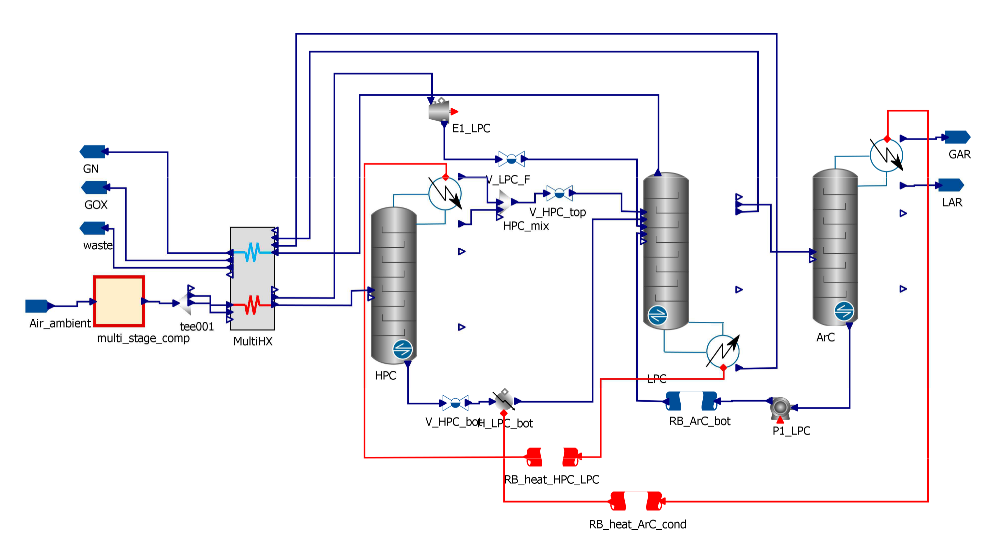
\includegraphics[width=0.9\textwidth]{Pictures/ASU_simple_gPROMS.eps}
            \caption{Implementation of simplified cryogenic air separation process in gPROMS.}
            \label{fig:ASU_simple_gproms}
        \end{figure}

        \Reffig{fig:ASU_simple_gproms} shows the flowsheet of the simplified ASU process depicted in \reffig{fig:ASU_simple_coco}.
        In order the symbols in the material streams (blue) and energy streams (red) represend so called recycle breakers, which
        play a vital role during initialization of the flowsheet. The recycle breakers play no part in the converged flowsheet.
        Their function is to break the recycle or feedback loops in the process and transform the process into a feed forward process
        during initial computations. To achieve that, the recycle breakers are supplied with initial guesses for for all properties
        associated with the respective material or energy streams. For the energy recycle breakers the transformation from open to
        closed operation mode is rather simple. The outlet energy stream is merely moved from initial guess to inlet stream by
        means of \refeq{eq:homotopy}. For the material breaker one hast to invest a little more effort, as not all properties can be
        moved so easily while maintaining physical sense. The material stream and pressure are treated identically, while the temperature
        needs to computed from an enthalpy balance.

        As for the concrete initialization procedure: first all recycle breakers are open and have the initial guesses at their outlet
        ports. Then all single units are converged. While this is done simultaneously in terms of the solution algorithm, the downstream
        units remain in the simplified stages of the unit respective initialization procedures wile the upstream units are solved with the
        rigorous models. Once all units have been converged, the recycle breakers are closed one after another. First the material stream
        between the Argon column (ArC) and the low pressure column (LPC), then the energy couple between the Argon condenser and
        and the oxygen rich material stream is closed. Finally the -- maybe most important -- connection between the LPC reboiler
        and HPC condenser is established.
